\chapter{行走} \label{chap:chap2}

\begin{figure}[!htb]
	\centering
	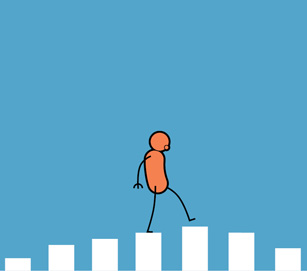
\includegraphics[width=0.5\linewidth]{chap2/2_0}
	% 加星号(*)表示不加编号
	\caption*{ \label{fig:2_0}}
\end{figure}

每走一步,你都会向前倾斜一点点,然后站稳,避免摔倒,一遍又一遍,你都在摔倒,然后站稳,避免摔倒。

\begin{flushright}
	——劳里$\cdot$安德森 \\
\end{flushright}

\begin{figure}[!htb]
	\centering
	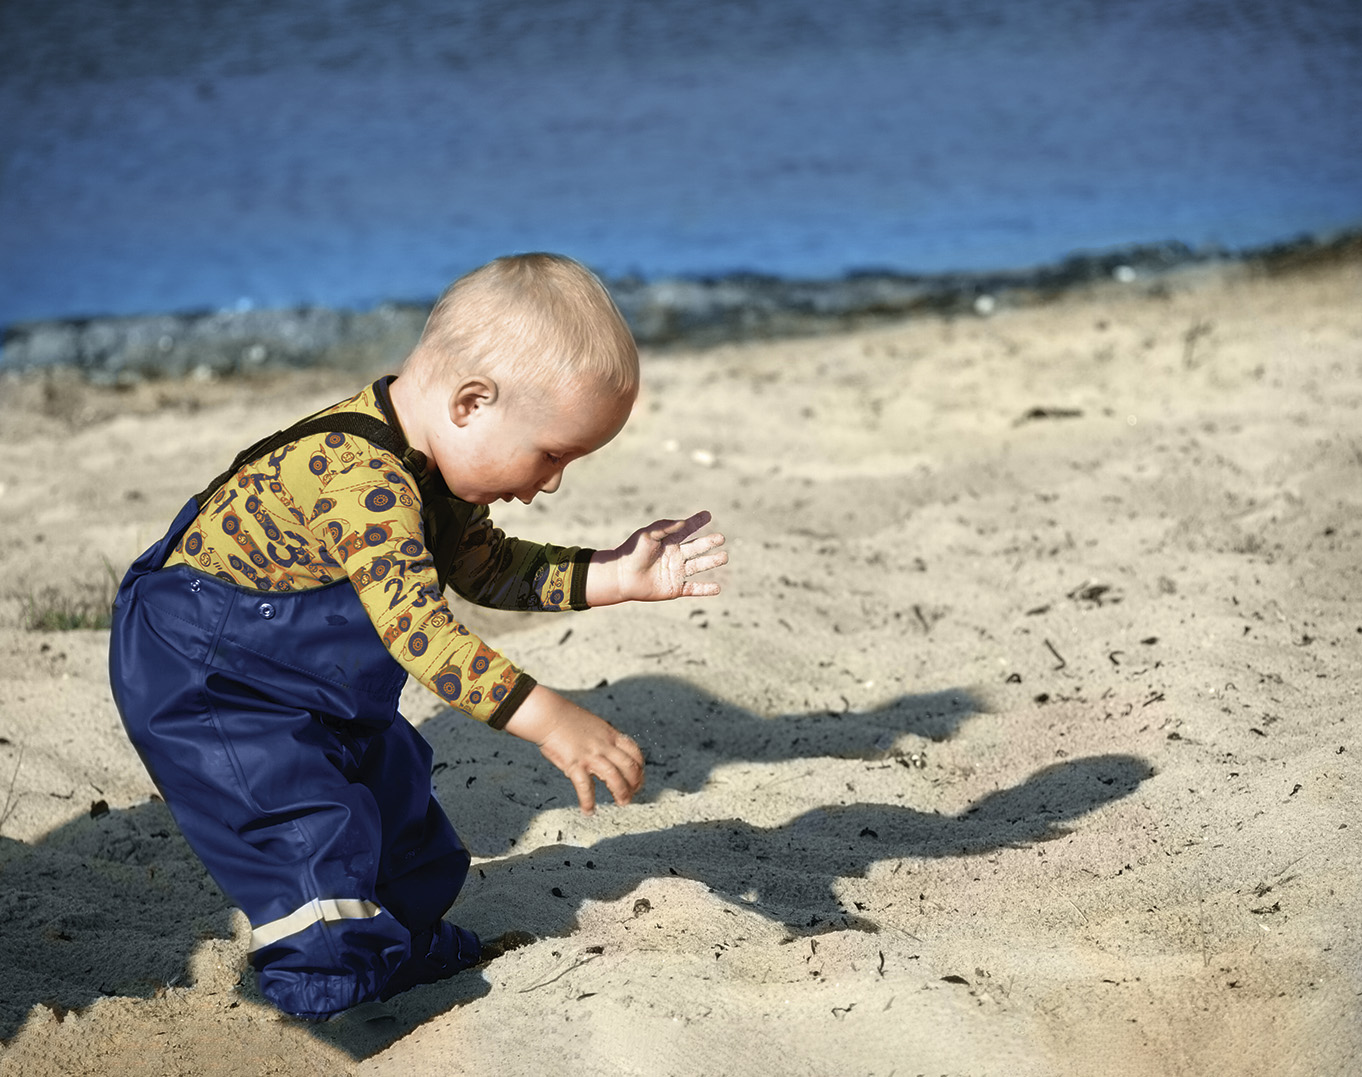
\includegraphics[width=0.5\linewidth]{chap2/2_0_2}
	% 加星号(*)表示不加编号
	\caption*{ \label{fig:2_0_2}}
\end{figure}

“有一天,我在月球上漫步,”
宇航员哈里森$\cdot$施密特兴高采烈地唱着,他即将踏上最后一次阿波罗任务的首次月球行走。
“在快乐的五月,”指挥官吉恩$\cdot$塞尔南附和道。
一缕缕月尘从他们的靴子上溅起,他们……究竟在做什么?跳跃?腾跃?跌跌撞撞?……穿过月球表面。


不管它是什么,它与我们通常认为的行走几乎没有什么相似之处。
施密特像个蹒跚学步的孩子一样慢步走着,左右摇晃。
塞尔南的步态看起来像个孩子骑着扫帚,却假装那是一匹马。
这两位训练有素的宇航员仿佛忘记了人类最基本的技能——行走——不得不学习一种新的移动方式(图~\ref{fig:2_1})。


\begin{figure}[!htb]
	\centering
	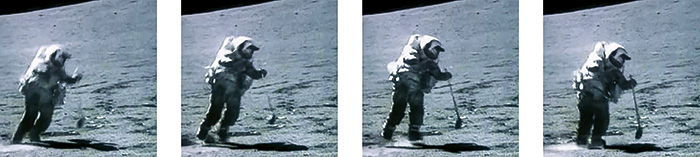
\includegraphics[width=1.0\linewidth]{chap2/2_1}
	\caption{宇航员很少在月球表面“行走”,他们更喜欢在月球引力下跳跃行走。
		图片由NASA提供。 \label{fig:2_1}}
\end{figure}


在本章中,我们将探讨为何看似简单的行走——人类进化已完美适应地球引力——在月球上却变得如此困难。
宇航员奇特的步态或许能帮助我们更充分地理解行走过程中发生的一系列精心安排的事件,以及引力在其中扮演的关键角色。


欣赏行走壮举的另一种方式是建造一台能够行走的机器。
塔德$\cdot$麦吉尔(Tad McGeer)的巧妙实验表明,一个拥有类似人类比例的无动力装置可以在倾斜的表面上行走。
这些装置无需大脑、脊髓或肌肉即可行走,只需在正确的方向上轻轻推一下即可。
这一观察表明,我们可以通过简单的机械模型来深入了解行走,我们将在本章中对此进行演示。


然而,在开始分析之前,有必要先了解一下步态周期以及运动中涉及的一些基本物理知识。
下一节将为你提供一些正确的方向。


\section{步行步态周期}

人类有两种常见的步态:行走和跑步。
我们都熟悉身体各部分在行走时所经历的典型周期性模式,但更正式地描述这些定性观察结果会很有帮助。
一个行走步态周期由同一条腿上连续两次的足部接触事件界定,另一条腿的足部接触通常发生在中途(图~\ref{fig:2_2})。
每条腿都有一个支撑期(此时足部接触地面)和一个摆动期(此时足部离地)。
支撑期始于足部接触地面,结束于足尖离地,对于一条腿而言,它占行走步态周期的约 60\%;其余时间则用于摆动。
由于支撑期比摆动期长,因此在每个行走步态周期中,都有双脚接触地面的时期,我们称之为双支撑期。
我们将只有一只脚接触地面的间隔称为单支撑期。


\begin{figure}[!htb]
	\centering
	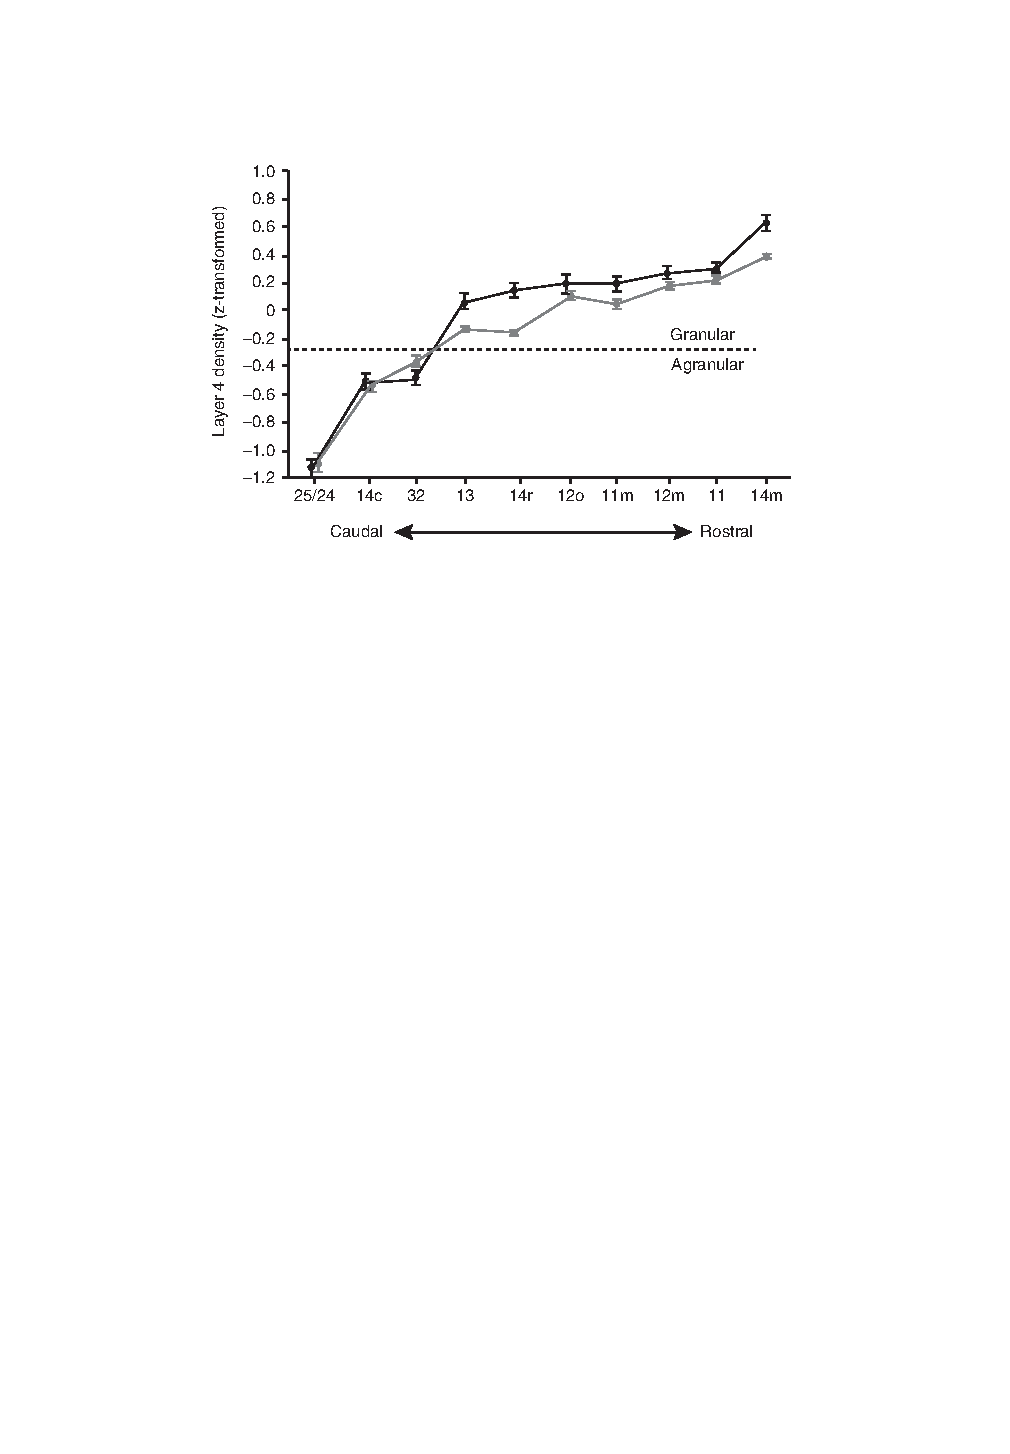
\includegraphics[width=1.0\linewidth]{chap2/2_2}
	\caption{步行步态周期及其组成事件(例如,脚接触)和阶段(例如,双支撑)。 \label{fig:2_2}}
\end{figure}


\textit{步长}是指两个连续足迹上同一点之间沿\textit{前进路线}的距离(图~\ref{fig:2_3})。
连续两步所走的距离,或一个步态周期所走过的距离,称为步长。
足部接触事件发生的速率(相当于步长持续时间的倒数)称为步频或步频;
迈步的速率称为步频。
步行速度可以用步长与步频的乘积来计算,或者也可以用步长与步频的乘积来计算:


\begin{figure}[!htb]
	\centering
	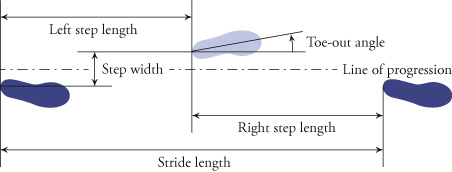
\includegraphics[width=0.8\linewidth]{chap2/2_3}
	\caption{水平(地面)平面上的步态测量。 \label{fig:2_3}}
\end{figure}

\begin{equation}
	\text{速度} = \text{步长} \times \text{步频}
			    = \text{步长} \times \text{起落}
\end{equation}

个人通常的步行速度会因身高、体能和其他因素而异。
健康成年人在平地上通常选择以约 1.2-1.4 米/秒的速度行走,步频为 2 步/秒。
典型的\textit{步长}约为 0.6-0.7 米。


另外 2 个值得注意的指标是在水平面上测量的(图~\ref{fig:2_3})。
\textit{踏步宽度}是脚平放时脚后跟中点与另一条腿上相同点之间的距离,垂直于前进路线测量。
健康成年人的\textit{踏步宽度}约为腿长的 10\%。
如果腿长约为 1 米,步宽约为 10 厘米,但对于正在学习走路的幼儿和一些平衡能力较差的人来说,步宽会更大。
\textit{足前进角}是前进路线与连接脚后跟中点和第二个脚趾(即足部的长轴)的线之间的角度。
正和负的\textit{足前进角}分别称为外倾角和内倾角。
成年人的外倾度通常较小,约为 10 度,但这个值在患有肌肉骨骼或神经系统疾病的个体之间可能会有所不同。
例如,患有小脑性共济失调(会导致平衡障碍)的人可能会以更大的\textit{足偏脚}和\textit{踏步宽度}行走,以减少跌倒的风险。


\section{地面反作用力}

我们通过测量双脚与地面之间的力来研究行走(图~\ref{fig:2_4})。
我们将在第~\ref{chap:chap11}~章中学习更多关于行走过程中肌肉协调的知识;
目前,只需知道肌肉通过产生力来产生运动即可。
肌肉产生的“作用力”会导致地面对双脚施加“反作用力”。
行走过程中,可以使用测力板测量地面反作用力。
测力板是一种仪器,可以测量人在测力板上行走时在垂直方向、前后方向和左右方向受到的力。​​
地面反作用力很重要,因为它可以衡量身体重心在每个时刻的加速度。
我们可以使用牛顿第二定律将地面反作用力和其他外力与身体重心 (com) 的加速度联系起来:
\begin{equation}
	F_{\text{external}} - mg = m a_{\text{com}} \label{eq:2_2}
\end{equation}
其中 $F_{external}$ 是施加于身体的所有外力之和,$m$ 是身体的总质量,$g$ 是重力加速度,$a_{com}$ 是质心加速度。
值得花点时间思考一下上一句中“和”和“全部”这两个词的含义。
当双脚接触地面时,我们必须将施加于每只脚的力相加。由于公式~\ref{eq:2_2}~是矢量和,所以方向很重要。
双脚下方力的垂直分量支撑着身体的重量。
但是,正如您在图~\ref{fig:2_5}~中所看到的,前脚上的前后力往往会抵消后脚上的前后力;
也就是说,前脚充当了刹车的作用,阻止我们走得越来越快,而后脚则提供推进力。
如果没有施加外力(即 $F_{external} = 0$,则物体处于自由落体状态,其质心将以 $g = 9.81 m/s^2$ 的速度加速向地面坠落。



\begin{figure}[!htb]
	\centering
	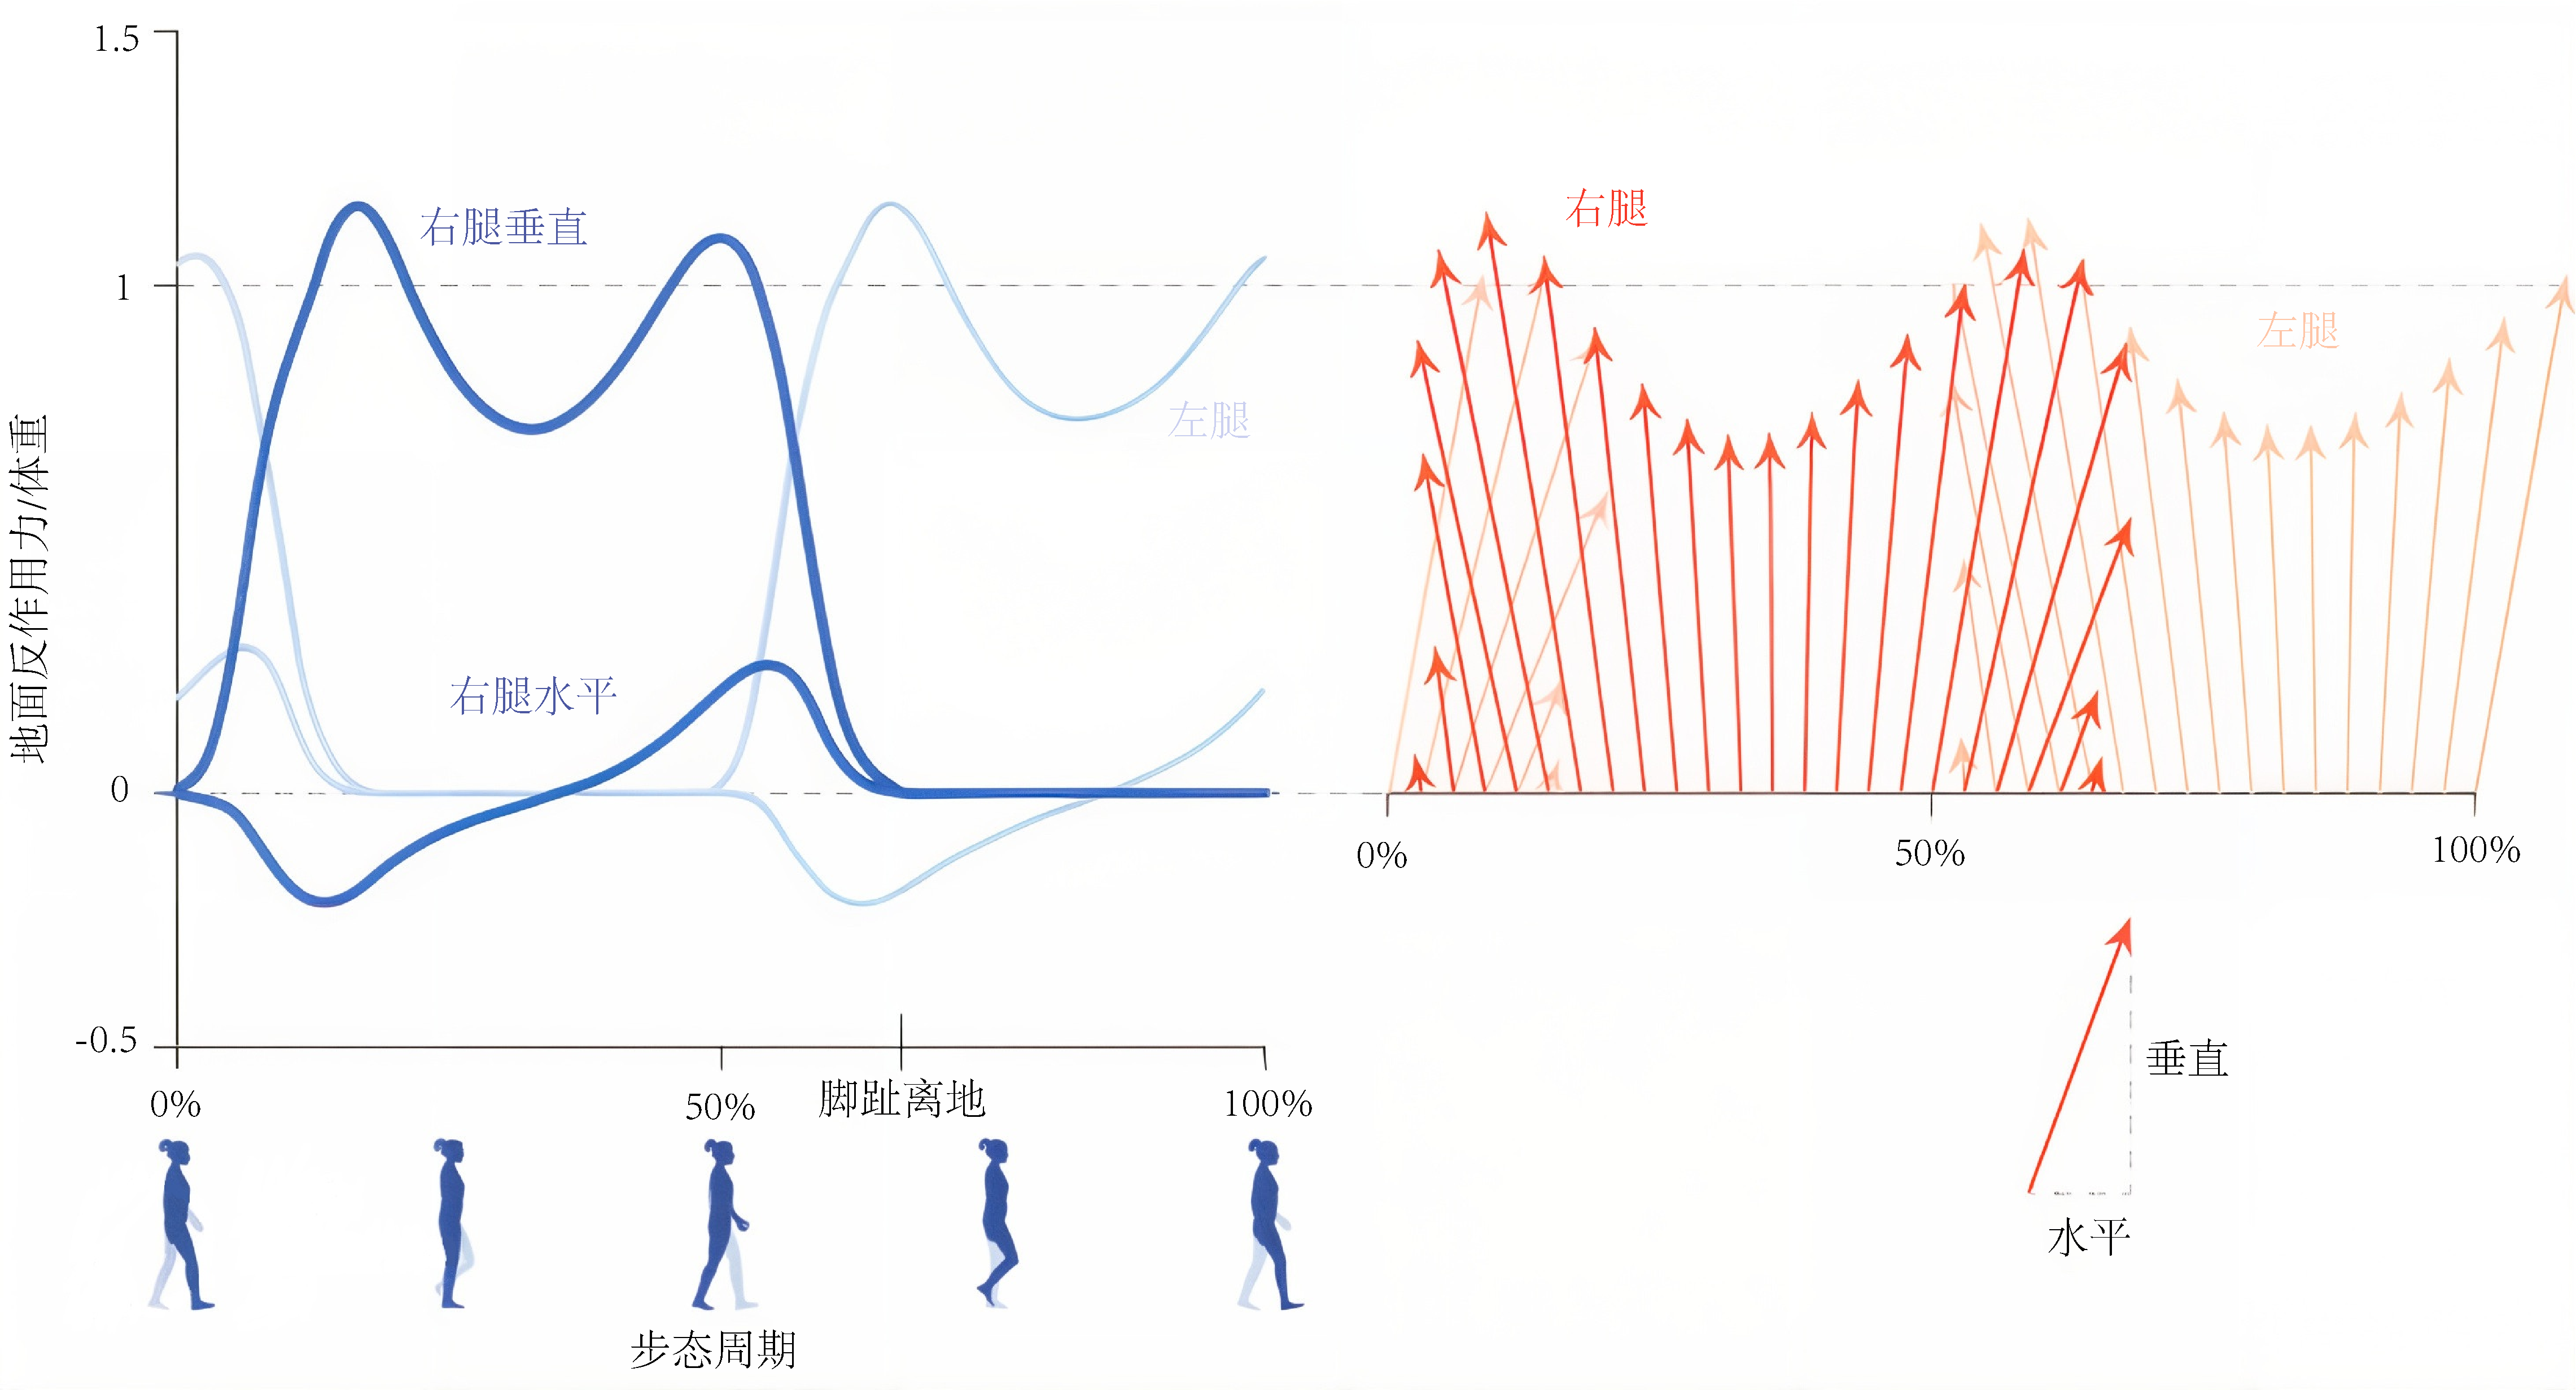
\includegraphics[width=1.0\linewidth]{chap2/2_4}
	\caption{以 1.55 米/秒的速度行走时代表性的地面反作用力。
		图中显示了步态周期内的垂直和水平(前后)分量(左)以及总矢量示意图(右)。
		正水平力指向前方。
		较小的左右力未显示。
		数据来自 Dembia 等人(2017)。 \label{fig:2_4}}
\end{figure}


\begin{figure}[!htb]
	\centering
	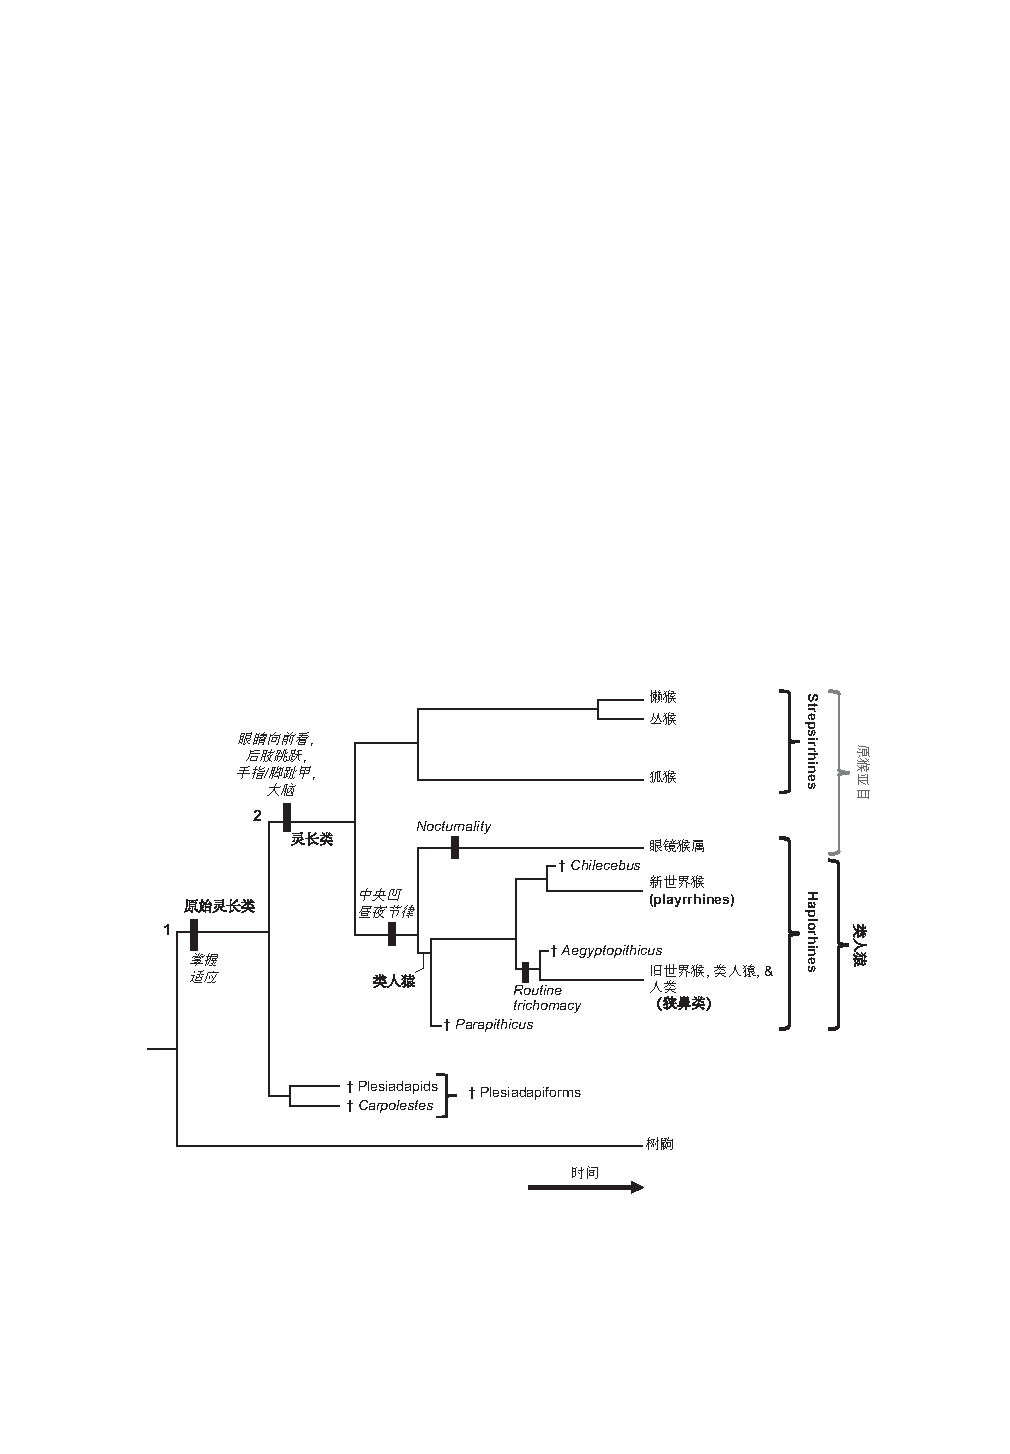
\includegraphics[width=0.9\linewidth]{chap2/2_5}
	\caption{以 1.55 米/秒的速度行走时,用两块测力板测量地面反作用力。
		两组箭头表示每只脚随时间推移受到的力。​​
		如黑色箭头所示,在双脚支撑时,地面反作用力的前后分量指向相反的方向。 \label{fig:2_5}}
\end{figure}


行走过程中地面反作用力的记录显示出几个有趣的特征(图~\ref{fig:2_6})。
地面反作用力的垂直分量在足部接触地面后迅速上升,并在步态周期的约 10\% 处达到大于体重的力。
在站立中期,垂直力降至低于体重,然后在蹬地时再次上升至高于体重。
然后,垂直力降至零,因为在脚趾离地后,足部不再接触地面。
平均而言,总垂直地面反作用力等于体重的 1 倍。
请注意,根据公式~\ref{eq:2_2},当地面反作用力的垂直分量等于体重时,重心没有净垂直加速度,恰好平衡了重力产生的向下力。

\begin{figure}[!htb]
	\centering
	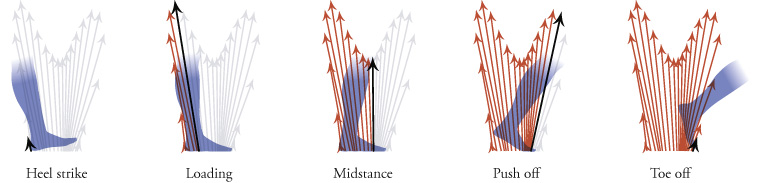
\includegraphics[width=1.0\linewidth]{chap2/2_6}
	\caption{以 1.55 米/秒的速度行走时,足部受到的典型地面反作用力。
		此处显示的力矢量(在空间中)与图~\ref{fig:2_4}~中显示的力矢量(随时间变化)相同。 \label{fig:2_6}}
\end{figure}


在站立的前半段,水平地面反作用力指向身体后部,使重心减速,之后指向身体前部。
除了图~\ref{fig:2_4}~所示的前后分量外,水平地面反作用力还有一个内外分量,这个分量虽然很小,但对于控制左右平衡很重要。
虽然在任何特定时刻重心都可能加速,但在几步匀速行走中,平均前后加速度为零。
改变前进速度时,平均前后加速度将不为零。
在垂直方向上,改变坡度时会出现非零平均加速度,例如从平地走到斜坡上时。


请记住,在步态周期的某些阶段,双脚都会接触地面,两个力相加,形成作用于身体的净向上力(图~\ref{fig:2_5})。
一个地面反作用力指向上方和前方,另一个指向上方和后方。
净地面反作用力主要指向上方,在双脚支撑阶段开始时有一个较小的向前分量,在脚趾离地时有一个较小的向后分量。
这些力抵消了向下的重力,并帮助您调节步行速度。


可以将测力板记录除以身体总质量,以估算质心加速度(公式~\ref{eq:2_2}~中的 $a_{com}$)。
该加速度可以积分一次以估算质心速度 ($v_{\text{com}}$),积分两次以估算其位置 ($r_{com}$)。
根据这些量,可以估算出质心向前的动能 ($E_{kf}$),其公式如下:
\begin{equation}
	E_{kf} = \frac{1}{2} m v_{\text{com}}
		   = \frac{1}{2} m 
		   	 ( \int a_{\text{com},f} (t) dt )^2  \label{eq:2_3}
\end{equation}
%
其中“$f$”下标表示前向分量
(请注意,垂直方向的速度波动非常小,因此我们在此忽略它)。
公式~\ref{fig:2_3}~中的积分符号提醒我们,加速度的影响是累积的,如果我们想要知道速度或动能,就必须将其随时间积分。
前向动能在站立中期最低,因为在站立的前半段,水平地面反作用力向后,使重心减速。
重力势能可以估算为:
\begin{equation}
	E_{\text{pg}} 
		= m g r_{\text{com},\text{v}} \label{eq:2_4}
\end{equation}
%
其中“v”下标表示垂直分量。
重力势能在站立中期达到最高,此时身体跨过站立肢(图~\ref{fig:2_7})。
如果我们绘制步态周期中的前向动能和重力势能,我们会发现它们是异相的(图~\ref{fig:2_8}):
当重力势能接近最小值时,前向动能达到峰值,反之亦然。
因此,总能量几乎保持不变。
我们在行走过程中保存能量的方法之一是用重力势能换取前向动能或前向速度,类似于在重力影响下摆动的钟摆的情况。
这一观察结果表明重力与行走有很大关系。


\begin{figure}[!htb]
	\centering
	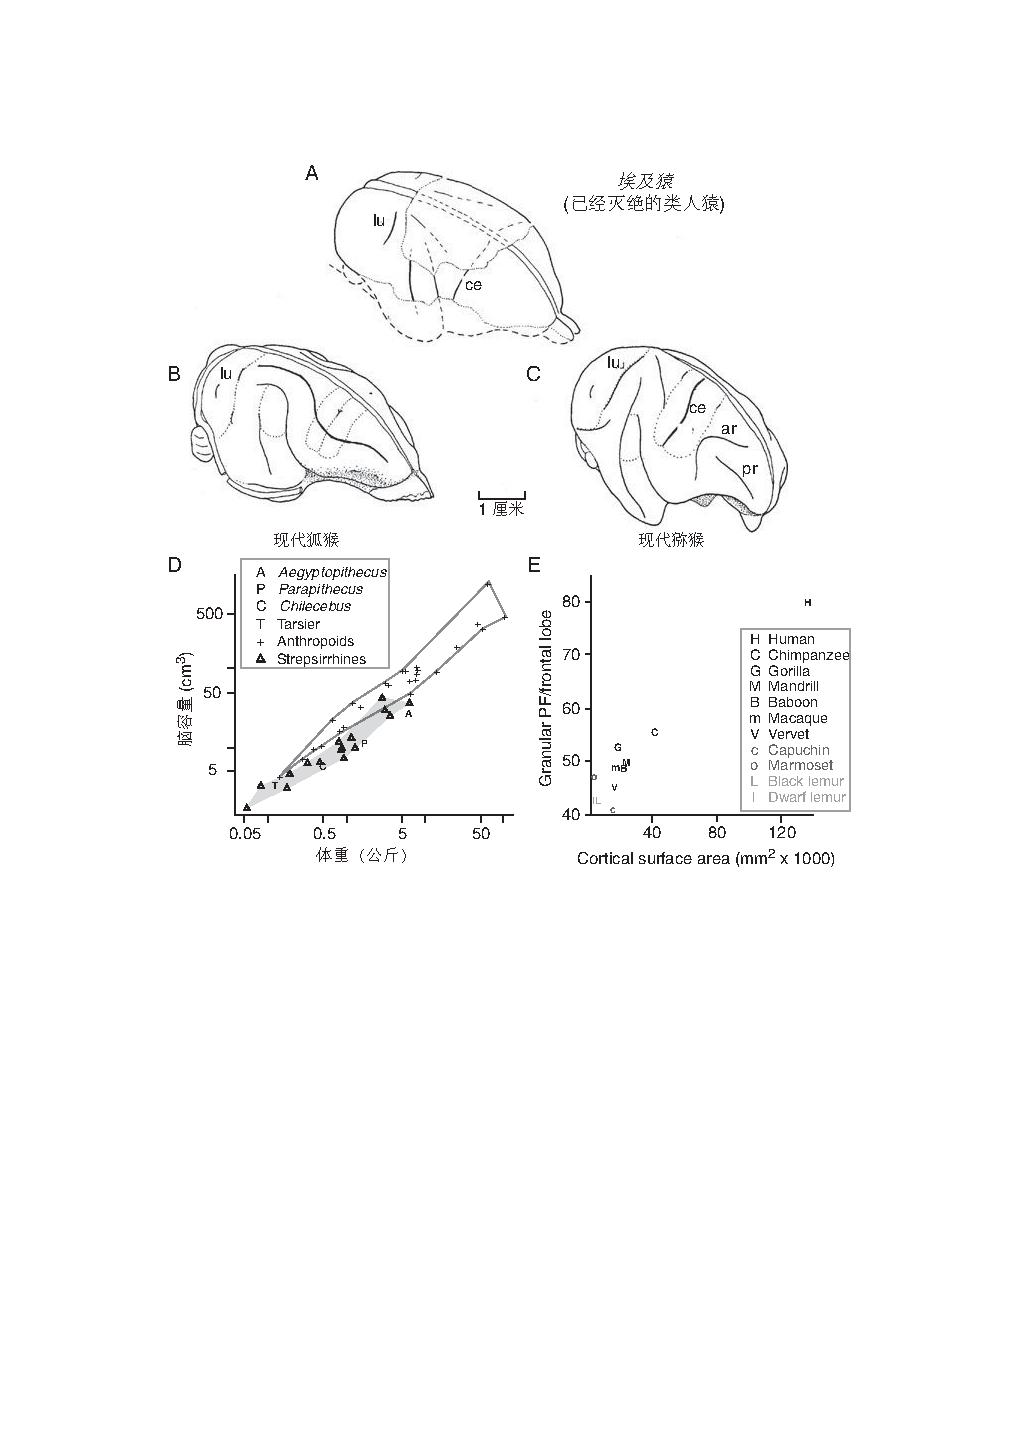
\includegraphics[width=0.5\linewidth]{chap2/2_7}
	\caption{一个步行步态周期内重心的垂直运动。 \label{fig:2_7}}
\end{figure}


\begin{figure}[!htb]
	\centering
	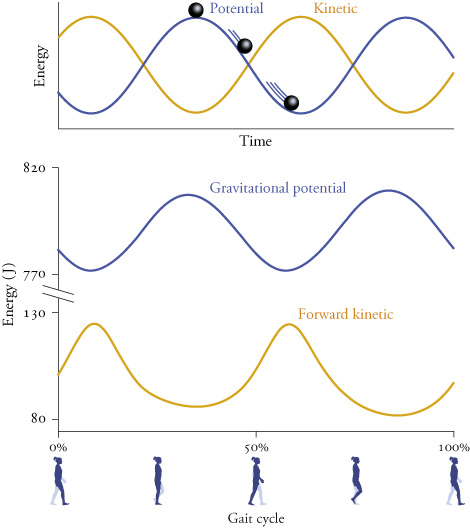
\includegraphics[width=0.8\linewidth]{chap2/2_8}
	\caption{以 1.55 米/秒的速度行走时,代表性重力势能和前向动能(下图)类似于球体在山坡上滚动时势能和动能的交换(上图)。
		行走过程中,垂直方向的动能波动较小,因此未显示。
		人体数据改编自 Dembia 等人\cite{dembia2017simulating}。 \label{fig:2_8}}
\end{figure}


\section{弹道步行模型}

1980年,托马斯$\cdot$麦克马洪(Thomas McMahon)和西蒙$\cdot$莫雄(Simon Mochon)基于以下假设,开发了一个行走数学模型:身体将势能转化为动能,并最大限度地减少肌肉在摆动阶段的作用。
该模型非常简单,仅由三个刚性连杆和三个旋转(销)关节组成,值得注意的是,没有肌肉或运动(图~\ref{fig:2_9})。
支撑肢由一个倒立摆表示,该摆的踝关节固定在地面上,使肢体能够在矢状面上绕踝关节旋转;
支撑肢的膝盖被假设锁定在完全伸展的位置。
摆动肢被建模为一个双摆,大腿和小腿部分在膝盖处通过销连接。
两条腿在臀部处固定在一起,并具有真实的质量分布。
头部、手臂和躯干的质量被忽略,但它们的质量集中在臀部。


\begin{figure}[!htb]
	\centering
	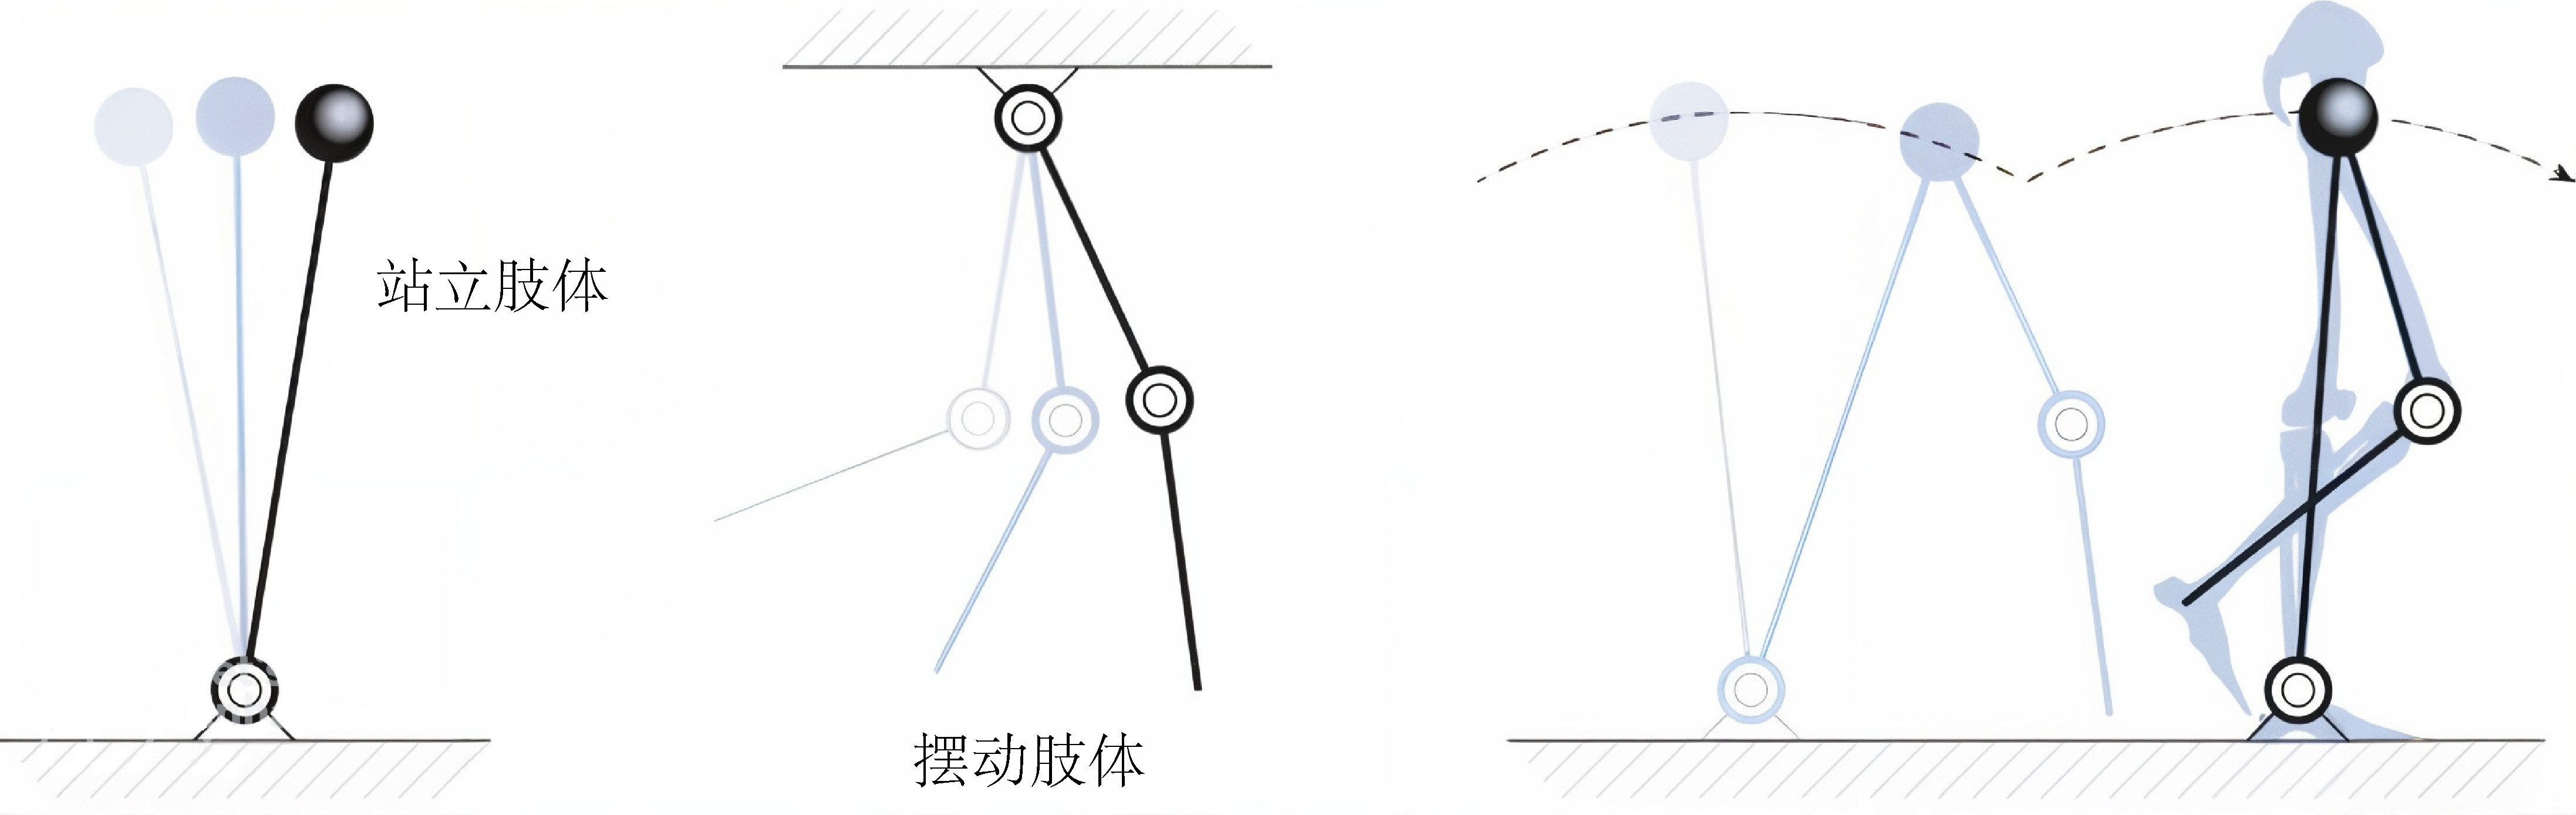
\includegraphics[width=0.8\linewidth]{chap2/2_9}
	\caption{Mochon 和 McMahon\cite{mochon1980ballistic}描述的弹道步行模型虽然简单,但分析能力强大。
		支撑肢用倒立摆(左)表示;
		摆动肢用双摆(中)表示。
		完整的模型是通过将两个肢体在髋部固定在一起而形成的(右)。 \label{fig:2_9}}
\end{figure}


肌肉活动的实验记录表明,在正常速度行走过程中,除了在摆动期的开始和结束时,摆动肢的肌肉相对不活跃。
因此,弹道步行模型假设肌肉完全被动地确定模型启动和完成摆动期所需的肢体节段的位置和速度,仅受重力作用(就像抛射物,因此称为“弹道”)。
当肌肉不活跃时,摆动肢的行为被认为类似于非受迫双摆。
如果在脚趾离地时为模型提供恰到好处的初始条件,则摆动肢的脚趾将在摆动中期离开地面,并且膝盖将在脚接触时完全伸展。


\section{弗鲁德数}

倒立摆本身是一个比弹道行走模型更简单的模型,它无法准确预测人类的步行速度,但确实提供了一些关于人类步行速度的物理限制的重要见解。
考虑一个倒立摆,如图~\ref{fig:2_9}~左侧所示,长度为 $l$,体重 $m$ 集中在臀部。
当臀部处于最大高度时,其瞬时速度 $v$ 水平方向,踝关节的垂直反作用力 ($F$) 等于向心力:
%
\begin{equation}
	F = \frac{m v^2}{l}
\end{equation}
% 
向心力是必须施加在摆锤上,以防止其离开地面的向下力。
由于地面无法对脚施加向下的力(除非你踩到胶水),所以向心力必须由体重 $mg$ 产生。
将这些力相等,并解出速度,我们发现倒立摆模型的最大行走速度 ($v_{max}$) 为
%
\begin{equation}
	v_{\text{max}} = \sqrt{g l}
\end{equation}

我们用$v_{max}$来定义无量纲步行速度($v^{*}$):
\begin{equation}
	v_{*} = \frac{v}{v_{max}}
\end{equation}
%
当速度超过 $v_{max}$ 时,脚会离开地面;因此,$0 \leq v^{*} \leq 1$,此时我们行走时就像一个倒立摆。
弗劳德数 ($F_r$) 是一个无量纲量,表示向心力与重力之间的比率:
%
\begin{equation}
	F_r = \frac{v^2}{g l}
		= (v^{*})^2
\end{equation}
%
无量纲步行速度和弗劳德数为比较不同最大速度和腿长的动物和人的步行速度提供了非常有用的指标。


倒立摆模型的一个重要预测是,如果 $l$ 或 $g$ 减小,最大步行速度也会减小。
当观察一个孩子与一个成年人并肩行走时,第一个关系很明显。
由于腿较短,孩子的弗劳德数会比成年人高,因此 $v_{max}$ 会较低。
因此,您可能会观察到成年人以舒适的速度行走,而孩子则跑着跟上。 
$v_{max}$ 对重力 $g$ 的依赖性解释了宇航员在月球表面遇到的挑战。
由于月球上的重力仅为地球的六分之一左右,因此月球上的 $v_{max}$ 与地面上的值相同。
因此,正常的地球步行速度会导致宇航员离开月球表面。
因此,阿波罗 11 号宇航员尼尔$\cdot$阿姆斯特朗和巴兹$\cdot$奥尔德林大多以慢速行走,以保持双脚着地。
后来的宇航员采用了各种各样的跳跃步态。
有趣的是,登月任务前的实验表明,袋鼠跳是最有效的步态,但宇航员很少采用这种策略。



值得注意的是,人类和其他陆地动物通常不会在弗劳德数为 1 时行走;
它们会在弗劳德数约为 0.5 时从行走过渡到奔跑以节省能量。
一个重要的例外是大象,它是最大的陆地动物,当弗劳德数大于 1 时,它们的行走速度似乎比倒立摆模型允许的速度快得多 (Hutchinson 等人,2003)。
与往常一样,理论与观察之间的差异提供了学习的机会。
从 2003 年到 2010 年,John Hutchinson 及其同事研究了视频,并使用定制的测力板对大象进行了实验。
(它们必须是强大的测力板!)
Hutchinson 发现,尽管大象始终至少有一只脚着地,因此仍然是传统意义上的“行走”,但它在高速下会夸张地蹲下(图~\ref{fig:2_10})。
这种“格劳乔步态”以喜剧演员格劳乔$\cdot$马克斯(Groucho Marx)的名字命名,他推广了这种行走方式。
这种步态意味着腿部肌肉产生巨大的力量,重力势能和动能的交换与倒立摆行走模型不一致。
因此,大象的步态某种程度上是行走和跑步的混合体。
下一章将讨论行走和跑步的区别,以及另一种大型动物——霸王龙——是否能够奔跑,届时我们将更详细地解释这一概念。

\begin{figure}[!htb]
	\centering
	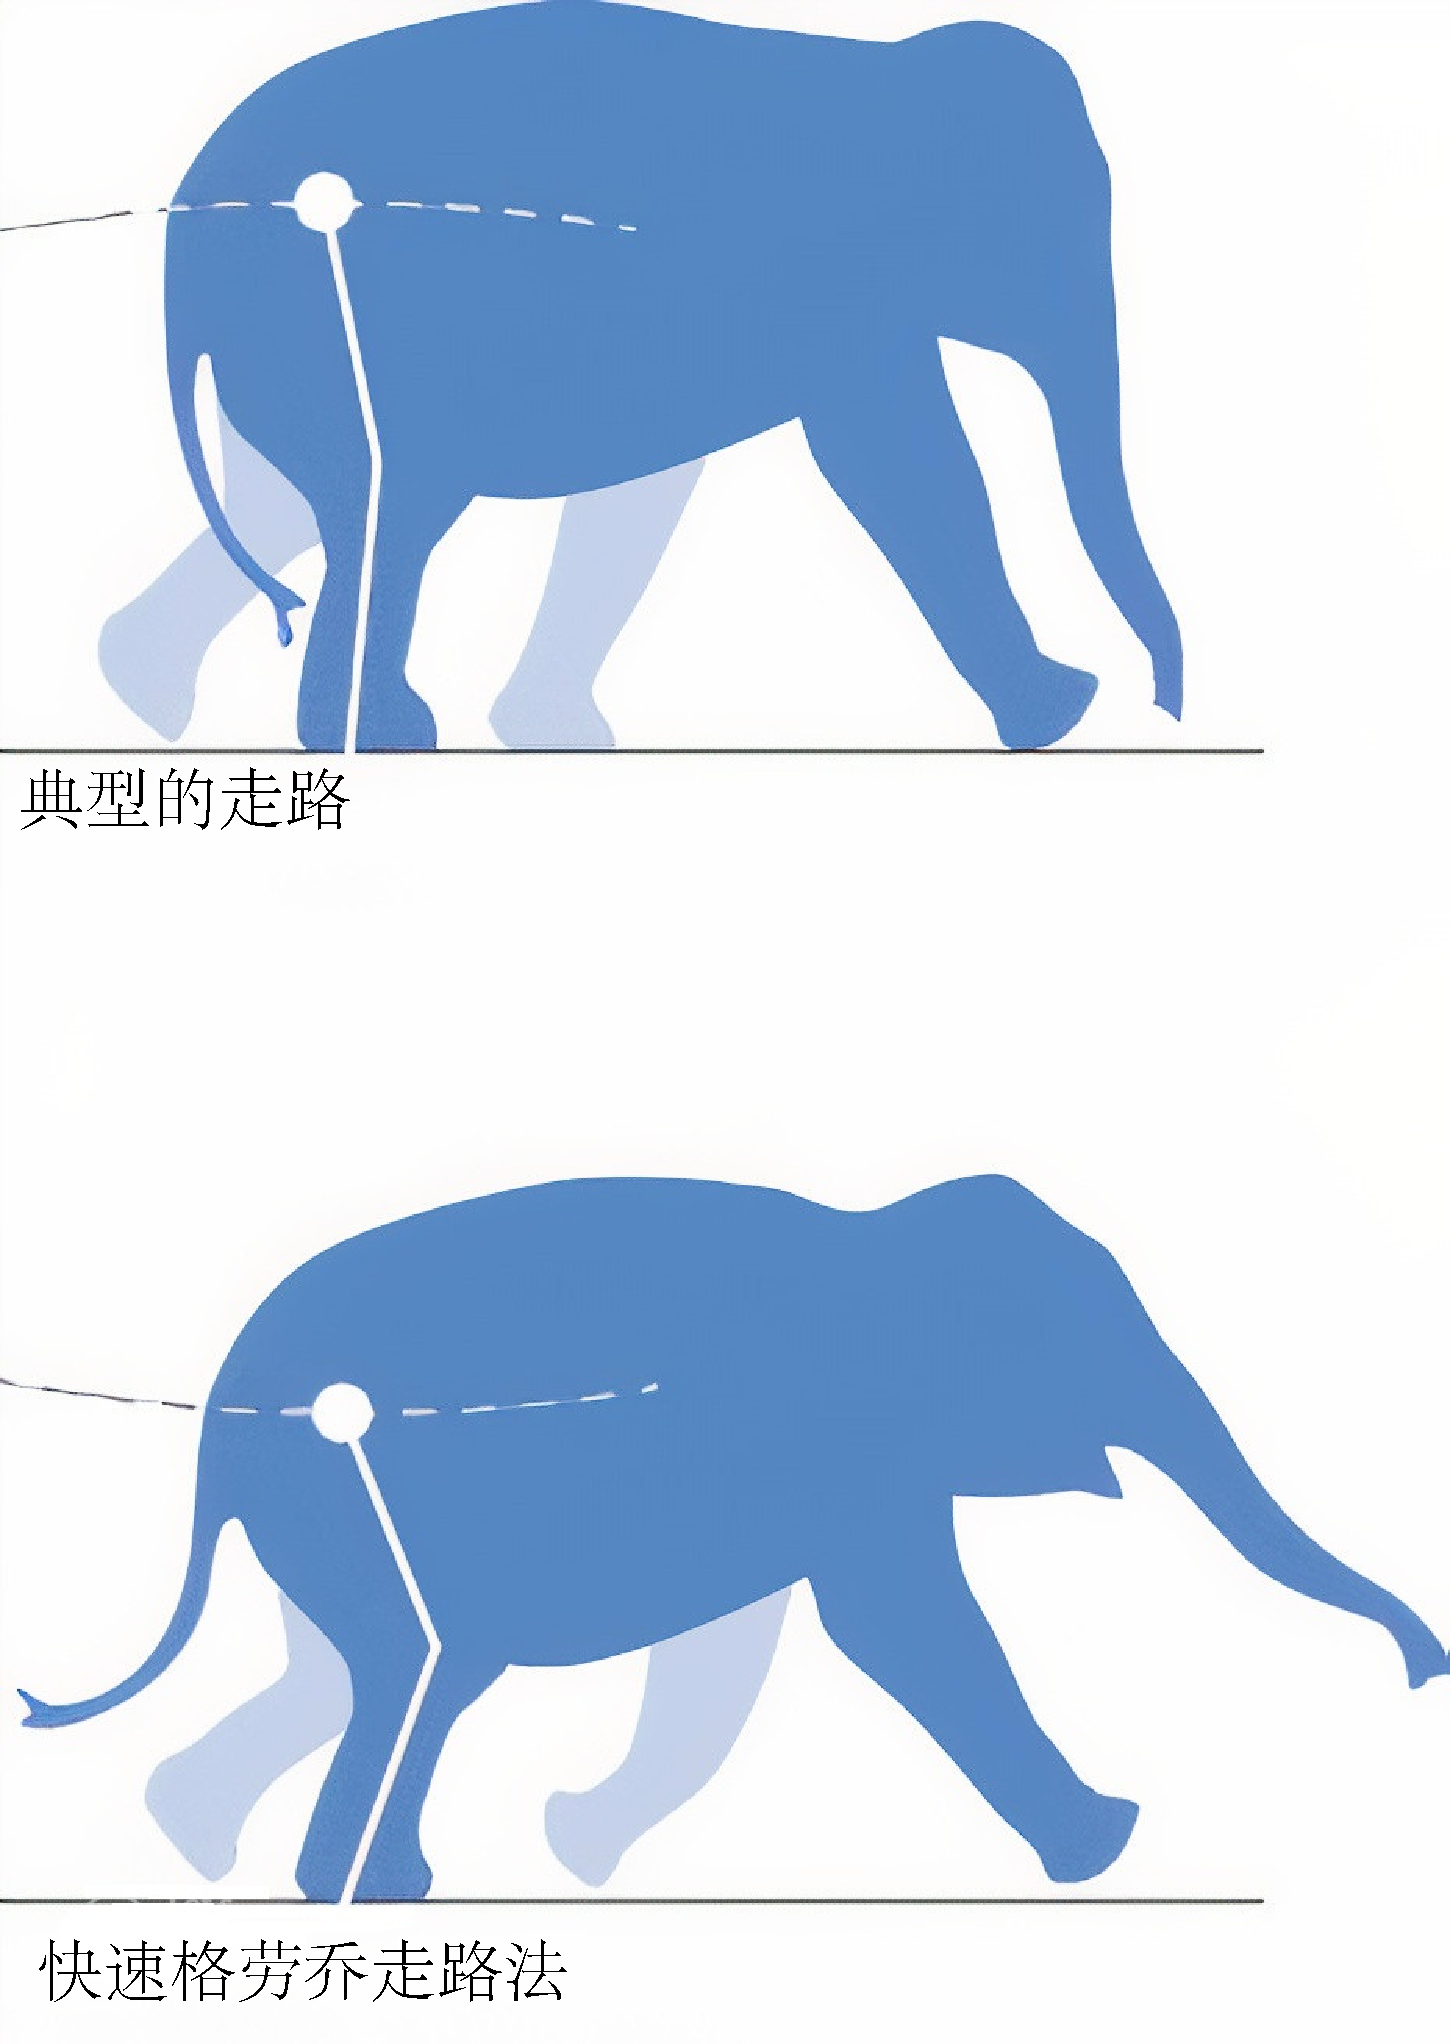
\includegraphics[width=0.4\linewidth]{chap2/2_10}
	\caption{即使在比赛中,大象也总是至少有一只脚着地,但步态(下图)比普通的行走(上图)更有弹性。
		这种步态通常被称为“格劳乔行走”,因格劳乔$\cdot$马克思而闻名。 \label{fig:2_10}}
\end{figure}


\section{运输成本}

弹道步行模型捕捉到了正常步行的一些显著特征,部分原因是我们自然而然地学会了如何以最小化能量消耗的方式移动。
减少腿部摆动时的肌肉活动就是一个例子。
我们也会自然地选择步行速度、节奏、步宽和其他变量,以最小化传输成本或移动给定距离所需的能量(图~\ref{fig:2_11})。
过去 60 年来的许多研究已经证实,我们行走的方式可以最小化传输成本——这是生物力学的一个重要原则。
步行的传输成本通常是通过收集和分析一个人以特定速度行走时吸入和呼出的混合气体来估算的(图~\ref{fig:2_12})。

\begin{figure}[!htb]
	\centering
	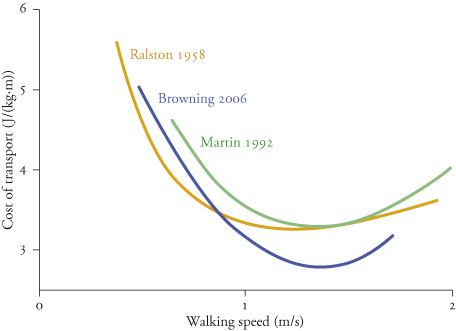
\includegraphics[width=0.75\linewidth]{chap2/2_11}
	\caption{运输成本随步行速度而变化。
		3 项实验研究表明,在自然步行速度附近,移动单位质量物体单位距离所需的能量最低。
		数据来自 Ralston\cite{ralston1958energy}、Browning 等人\cite{browning2006effects}和 Martin 等人\cite{martin1992effects}。 \label{fig:2_11}}
\end{figure}

\begin{figure}[!htb]
	\centering
	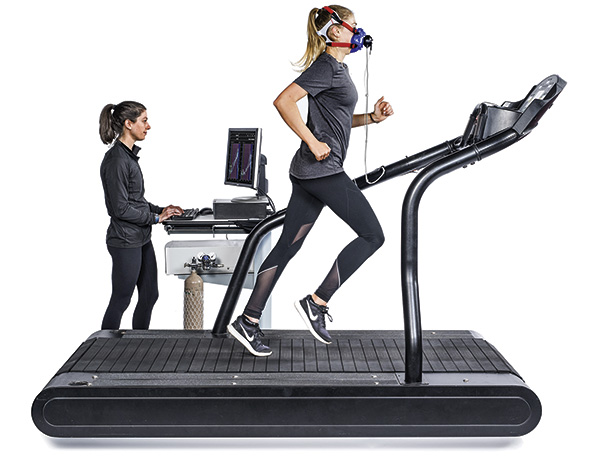
\includegraphics[width=1.0\linewidth]{chap2/2_12}
	\caption{测量氧气消耗量和二氧化碳生成量,以计算跑步过程中消耗的能量的实验。
		该实验也用于计算步行过程中的运输成本,如图~\ref{fig:2_11}~所示。 \label{fig:2_12}}
\end{figure}


请注意,我们无法直接测量能量消耗,但基于呼吸测量的间接估算是一个很好的替代方法。
我们的肌肉由燃烧碳水化合物、脂肪和蛋白质的化学反应提供动力。
这些反应消耗氧气并产生二氧化碳。通过确定废气产生的速率,我们可以推断出使用了多少燃料,从而消耗了多少能量。
如图~\ref{fig:2_11}~所示,我们通常将运输成本表示为每公斤体重移动一米所需的焦耳能量。



虽然弹道模型有助于理解行走的一些基本特征,但它也存在一些局限性。
例如,它无法模拟双支撑,而这对于理解连续步伐之间的过渡至关重要。
倒立摆模型预测我们的最大行走速度将发生在弗劳德数为 1 时,而实际上人类在弗劳德数远低于 1 时从行走过渡到跑步,竞走运动员在弗劳德数大于 1 时可以“行走”。
还要注意,弹道步行模型可能会让人得出结论,认为行走不会消耗任何能量。
此外,具有刚性站立肢的模型无法准确预测实验观察到的地面反作用力。
最后,弹道步行模型不会产生重复的步态周期。
其中一些限制在一个稍微复杂一些的模型(称为动态步行模型)中得到了解决。


\section{动态步行模型}

弹道行走模型在钟摆模型的基础上,通过增加膝盖(或者更准确地说,一个膝盖)进行了改进。
我们或许会认为,再增加一个解剖学元素就能进一步改进模型。
但它的作用远不止于此:
通过增加双脚,塔德$\cdot$麦吉尔设计了一个可以在实验室中制造和测试的行走机器人。


麦吉尔曾接受过航空工程师的培训,因此他采用的策略与一个世纪前飞机研发的策略如出一辙也就不足为奇了。
在尝试动力飞行之前,莱特兄弟多年来一直致力于研发利用滑翔机下坡时重力势能驱动的滑翔机。
到1902年底,他们已经完成了数百次此类飞行。
莱特兄弟掌握了滑翔技术后,便自信满满地掌握了动力飞行,并于次年完成了首次动力飞行记录(Collins 等人,2005)。


效仿莱特兄弟,在莫雄和麦克马洪提出弹道模型十年后,麦克吉尔构建了一种被动机构,在适当的初始条件下,该机构可以仅靠重力驱动,稳定地从缓坡上行走(图~\ref{fig:2_13})。
证明这种机构的可构建性是一项突破,并开启了“动态行走”研究的新领域,动态行走主要由腿部的被动动力学产生运动。
如今,动力驱动的动态步行机器人的设计遵循莱特兄弟的原理:
如果被动机构能够严格在重力作用下从缓坡上移动,那么主动机构应该能够使用执行器在平地上移动,执行器仅注入重力在下缓坡时提供的少量能量。


\begin{figure}[!htb]
	\centering
	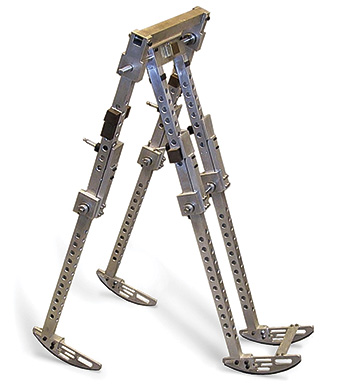
\includegraphics[width=0.6\linewidth]{chap2/2_13}
	\caption{塔德$\cdot$麦吉尔\cite{mcgeer1990passive}描述的步行机器的复制品。
		该装置包含两对腿,在给定正确的初始姿势和推力的情况下,能够沿着倾斜的表面行走。
		照片由史蒂夫$\cdot$柯林斯提供。 \label{fig:2_13}}
\end{figure}



动态步行模型在三个关键方面扩展了弹道模型:添加双脚、建模双支撑,以及最重要的,实现一步一步的过渡(图~\ref{fig:2_14})。
这些特性使该机构能够进行周期性、连续的步行。
在单支撑期间,支撑肢的脚在地面上滚动(不滑动),而摆动肢被动摆动。
膝关节伸展止动装置可防止摆动结束时膝关节过度伸展,并保持支撑肢完全伸展,被动支撑身体重量。
在支撑的前半段,重心向上移动,在后半段向下移动。
就在脚接触之前,支撑肢踝部产生的推离力矩将重心重新定向到向上的轨迹。
在脚接触之前重新定向重心可降低脚与地面碰撞的速度和相应的能量损失。
在脚与地面碰撞时以及膝盖完全伸展时撞到止动装置时,仍然会损失一些能量。
为了实现连续的步态,每一步都必须注入少量能量,以补偿能量的耗散以及关节的摩擦损失。
在完全被动的步行机中,这种能量由行走机构在缓坡下行时产生的重力势能提供;
在平地上,这种能量可以由位于踝部或臀部的电机注入。


\begin{figure}[!htb]
	\centering
	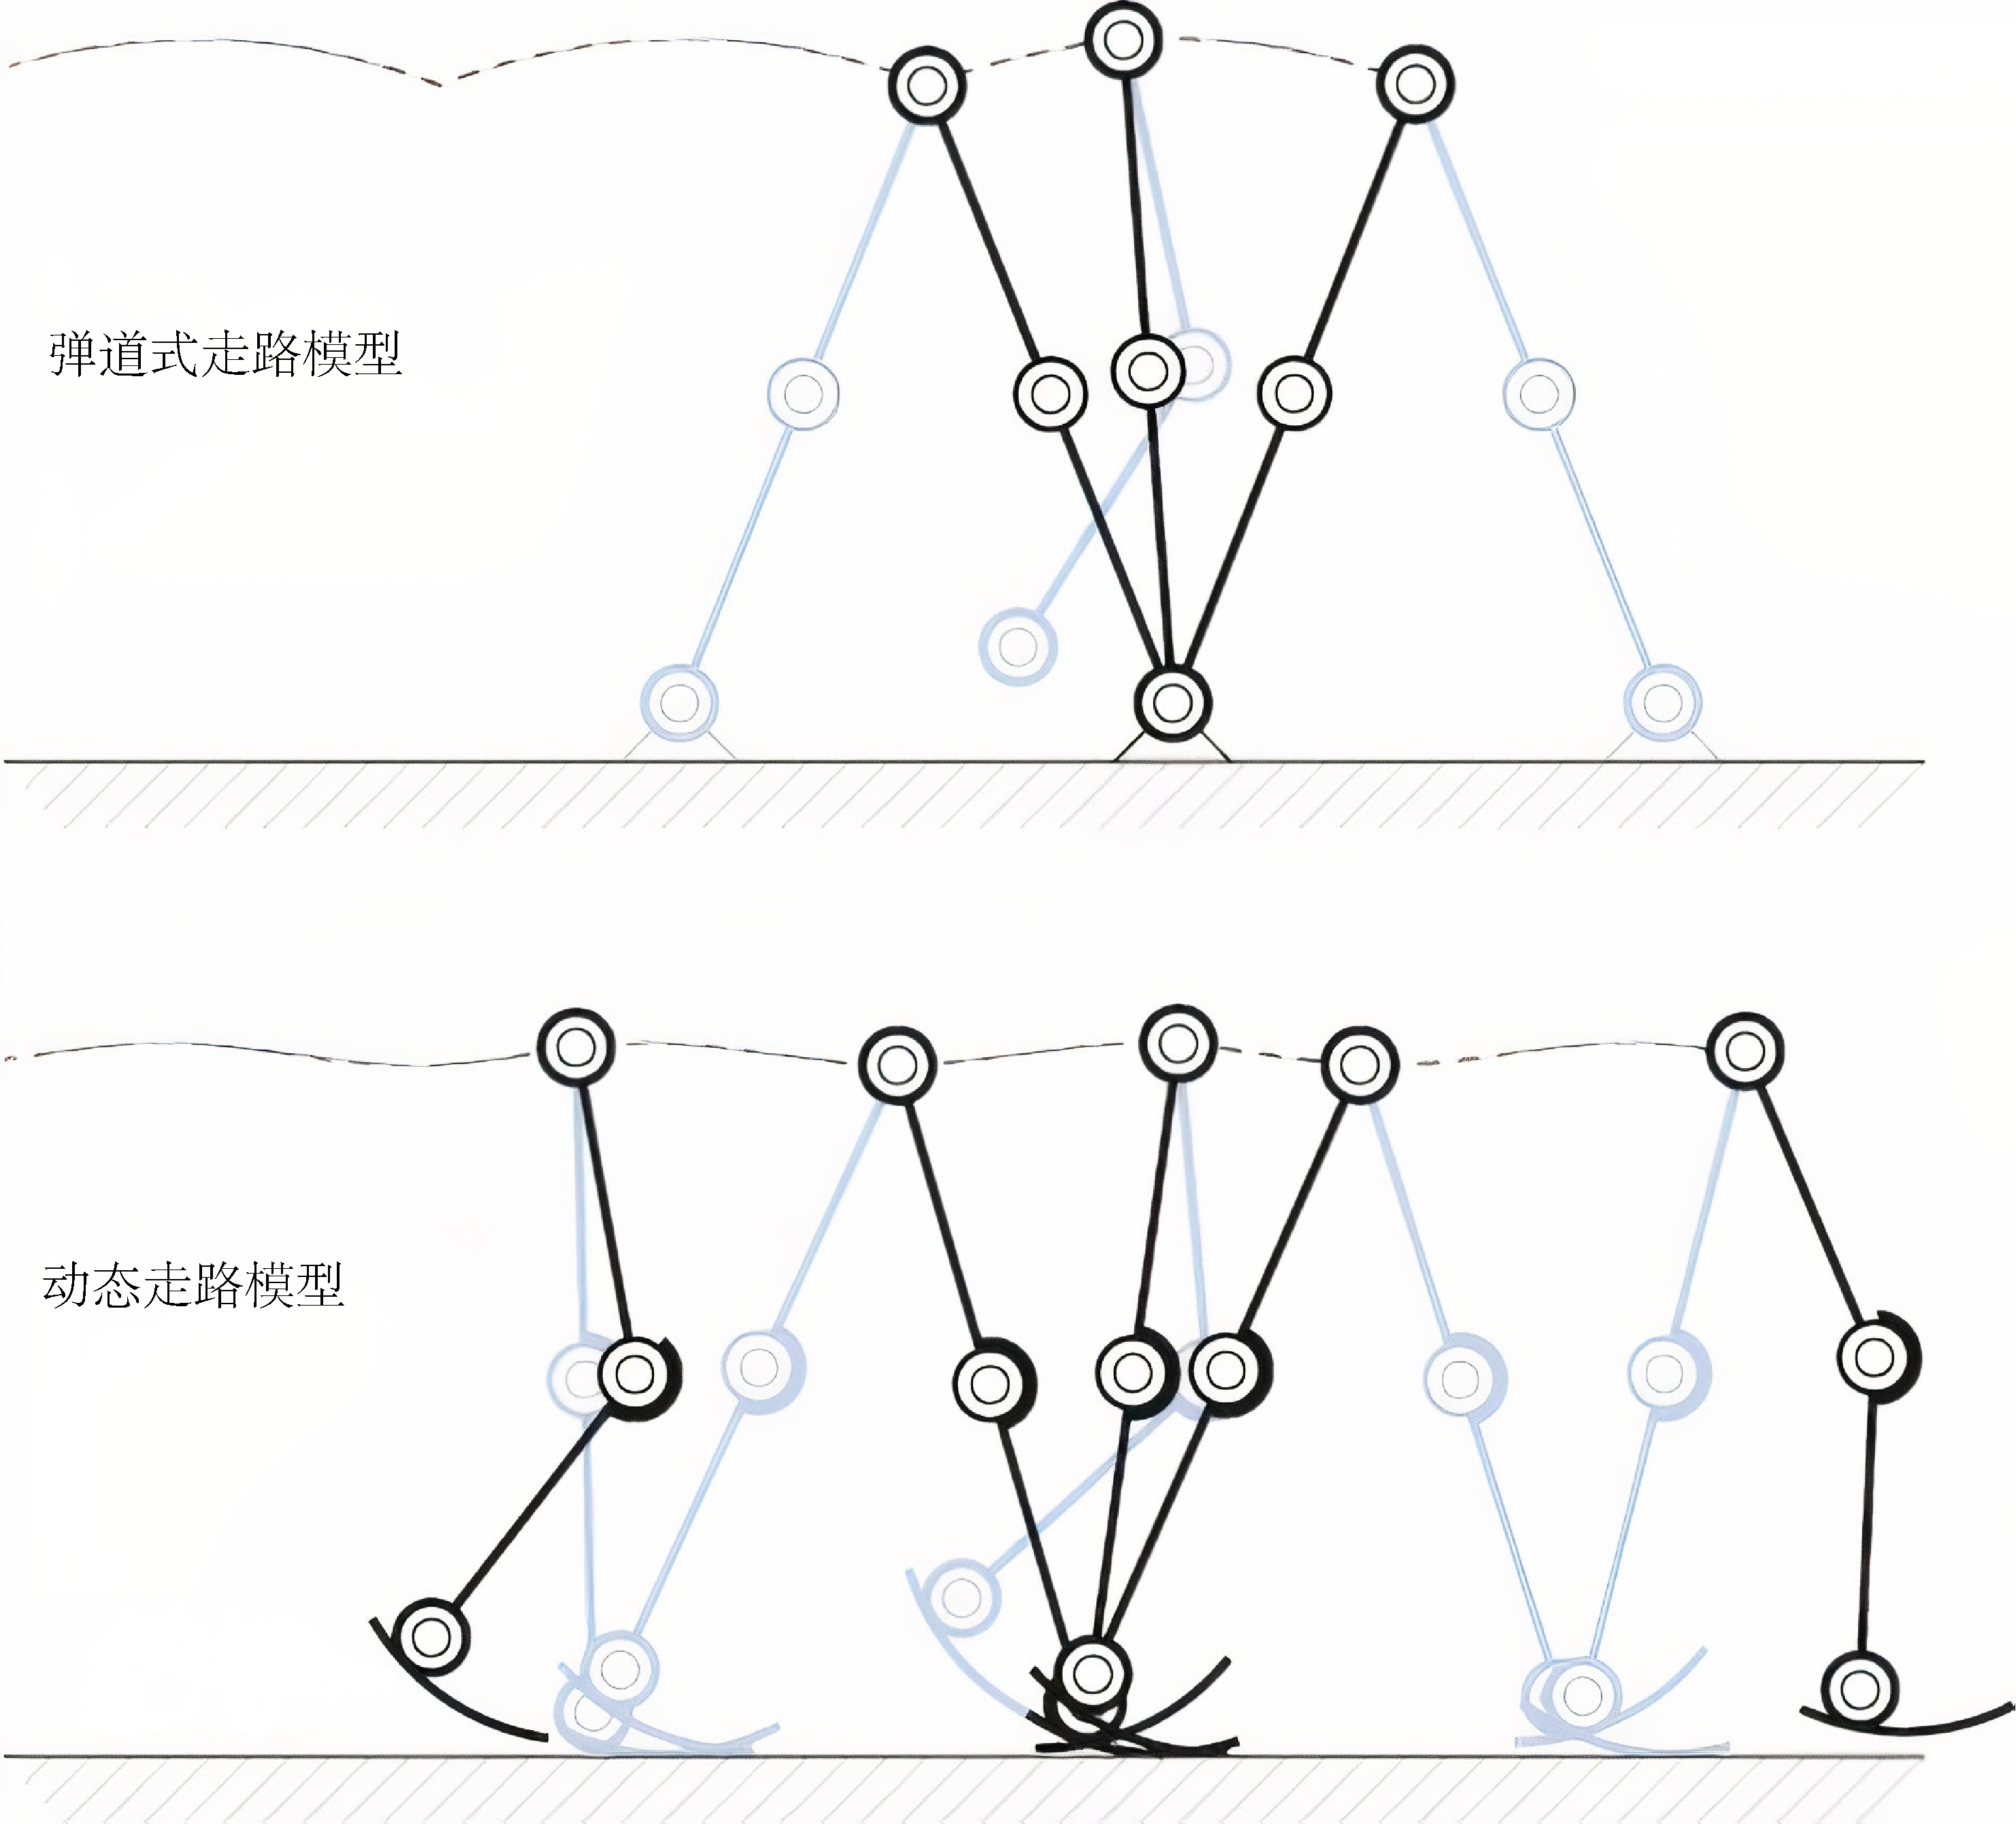
\includegraphics[width=0.6\linewidth]{chap2/2_14}
	\caption{Kuo\cite{kuo2010dynamic}描述的动态步行模型。
		该模型通过实现步进过渡,产生重复的步态周期,解决了弹道模型的一些局限性。 \label{fig:2_14}}
\end{figure}


动态步行模型为理解平地行走的一些基本特征提供了一个理论框架。
动态步行模型已用于研究步态周期中的能量消耗、能量消耗如何随步行速度而变化以及人类步行的其他方面。
例如,在开始双脚支撑时改变质心轨迹所需的能量称为步进转换成本。
动态步行模型正确地预测了该成本会随着步幅更大、速度更快而增加。
增加步长(同时保持步频恒定)会增加能量消耗,因为质心速度增加,其轨迹必须改变更大的幅度。
增加步频(同时保持步长恒定)也会增加能量消耗,因为腿部必须比单独由被动动力学产生的速度更快地摆动,而肌肉会消耗能量来摆动腿部。


步步过渡和腿部强制摆动运动所产生的能量消耗,除了维持平衡外,还会影响人类行走的成本。
人类通常会选择步长和步频,以最小化运输成本。
当步行速度超过运输成本最低的速度时,人类会以几乎等比例增加步长和步频,以平衡步步过渡和腿部强制摆动带来的成本增加。
步步过渡的成本也可以通过将我们的双脚像轮子的一部分一样使用(请注意图~\ref{fig:2_14}下方的弧形双脚)来降低,从而减少所需的重心方向变化。
当地面反作用力从脚接触时的后脚掌转移到脚趾离地时的前脚掌时(图 2.5),人类的双脚实际上在地面上滚动。
对于动态步行者来说,脚的位置至关重要:
如果脚的位置过于前倾,步行者就会向后摔倒;
如果腿部摆动速度过慢且步长过短,步行者就会向前摔倒。


动态步行模型比弹道模型具有更强的分析能力,但当然也存在局限性。
许多建模假设和简化使得该模型无法用于研究人类步行的某些要素。
例如,动态步行模型假设运动严格为平面运动,忽略了矢状面以外的运动。
McGeer 的装置通过将腿部数量增加一倍来最大限度地减少左右摇摆,从而强化了这一假设。
2001 年,当时就读于康奈尔大学的史蒂夫·柯林斯 (Steve Collins) 制造了第一台双足被动动态步行机(图~\ref{fig:2_15})。
设计这种机制需要仔细关注机器质心的轨迹,以防止其因非矢状面运动而跌倒。
矢状面上的反向摆动臂稳定了偏航,足部形状和侧向摆动臂控制了倾斜,而柔软的鞋跟则避免了对足部接触时姿势的敏感性(Collins 等人,2001)。
在每种情况下,仿生学都改善了机制的性能,并且让我们了解了为什么这些要素(手臂摆动、脚和脚跟)会给人类带来生物力学优势。


\begin{figure}[!htb]
	\centering
	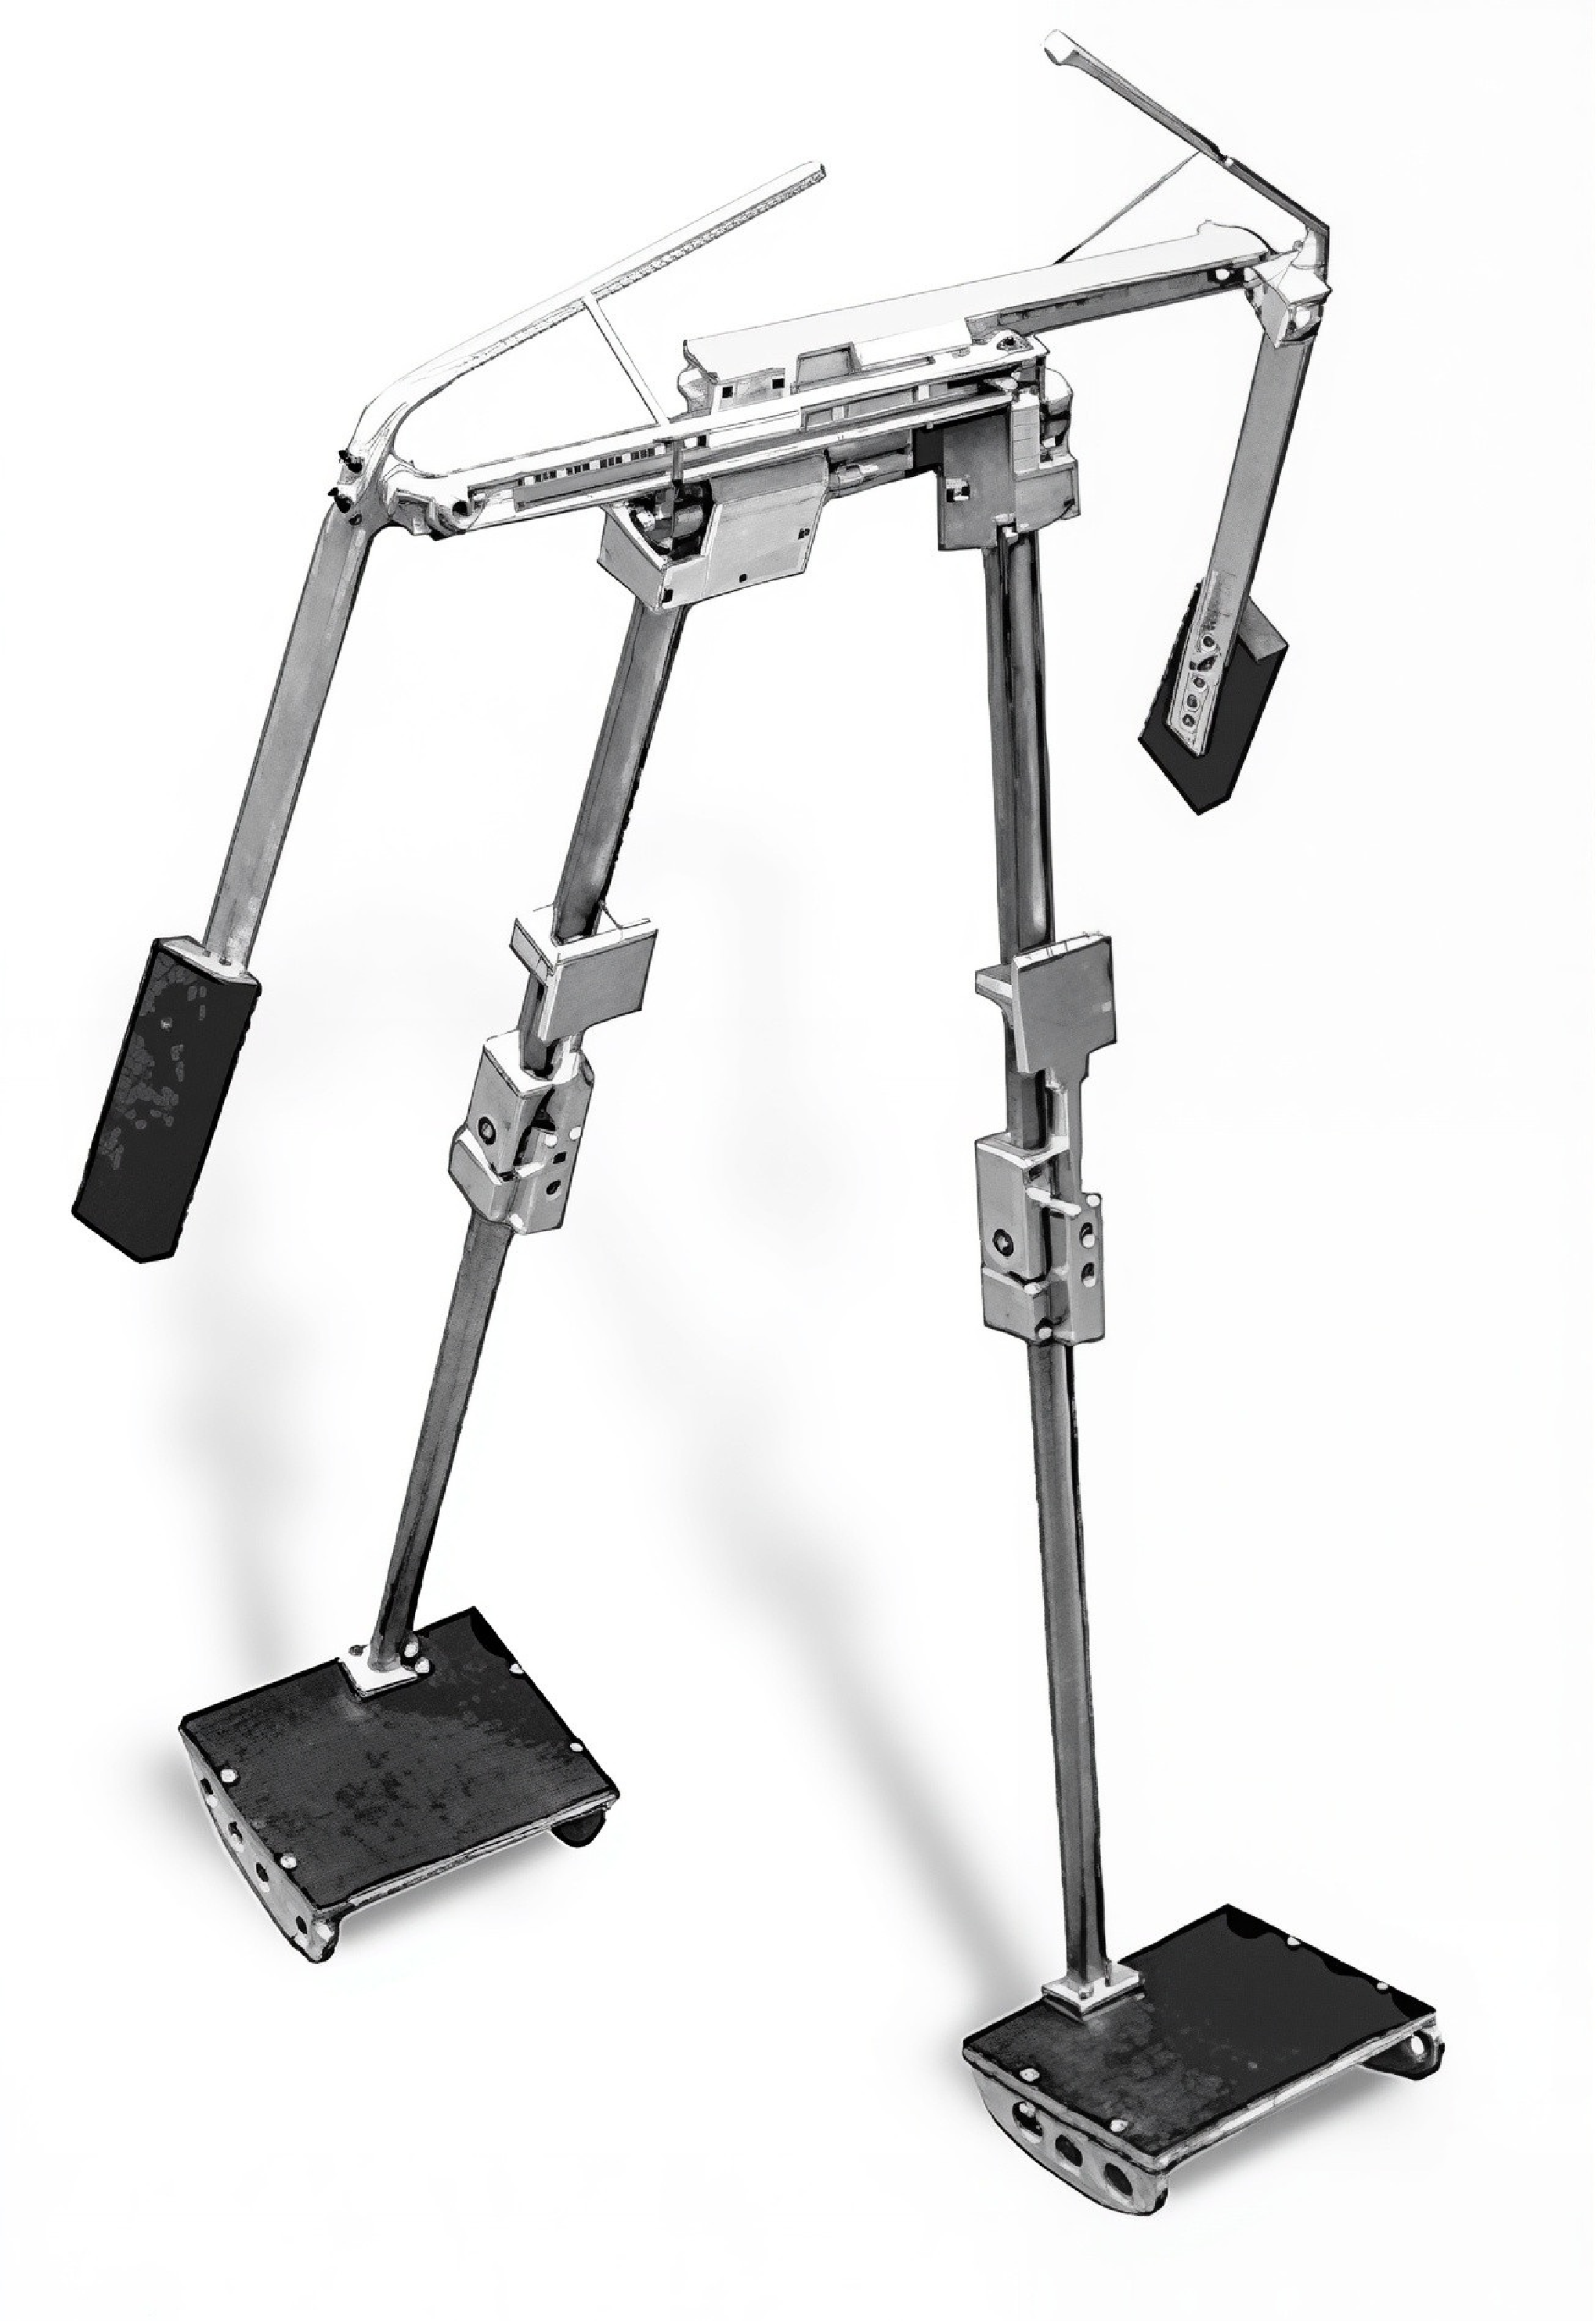
\includegraphics[width=0.45\linewidth]{chap2/2_15}
	\caption{首款双足被动式动态助行器。 \label{fig:2_15}}
\end{figure}


\section{手臂摆动}

到目前为止,我们已经使用了简单的模型来研究下肢的动力学,但上肢在行走中也发挥着作用。
上肢最明显的运动是手臂摆动,但我们行走时为什么摆动手臂却不那么明显。
为了研究这种行为,史蒂夫$\cdot$柯林斯和他的同事提出了一种类似于麦吉尔的直腿被动行走机制,但在臀部连接了一个类似手臂的摆锤(图~\ref{fig:2_16})。
他们测试了几种手臂摆动策略,包括我们熟悉的“正常”摆动,以及一种“反正常”摆动,即左臂随左腿前进,右臂随右腿前进。
我不禁将这种策略称为“兄弟步”,以纪念我的哥哥布莱恩$\cdot$德尔普,他小时候喜欢这样走路,我们俩都喜欢。


\begin{figure}[!htb]
	\centering
	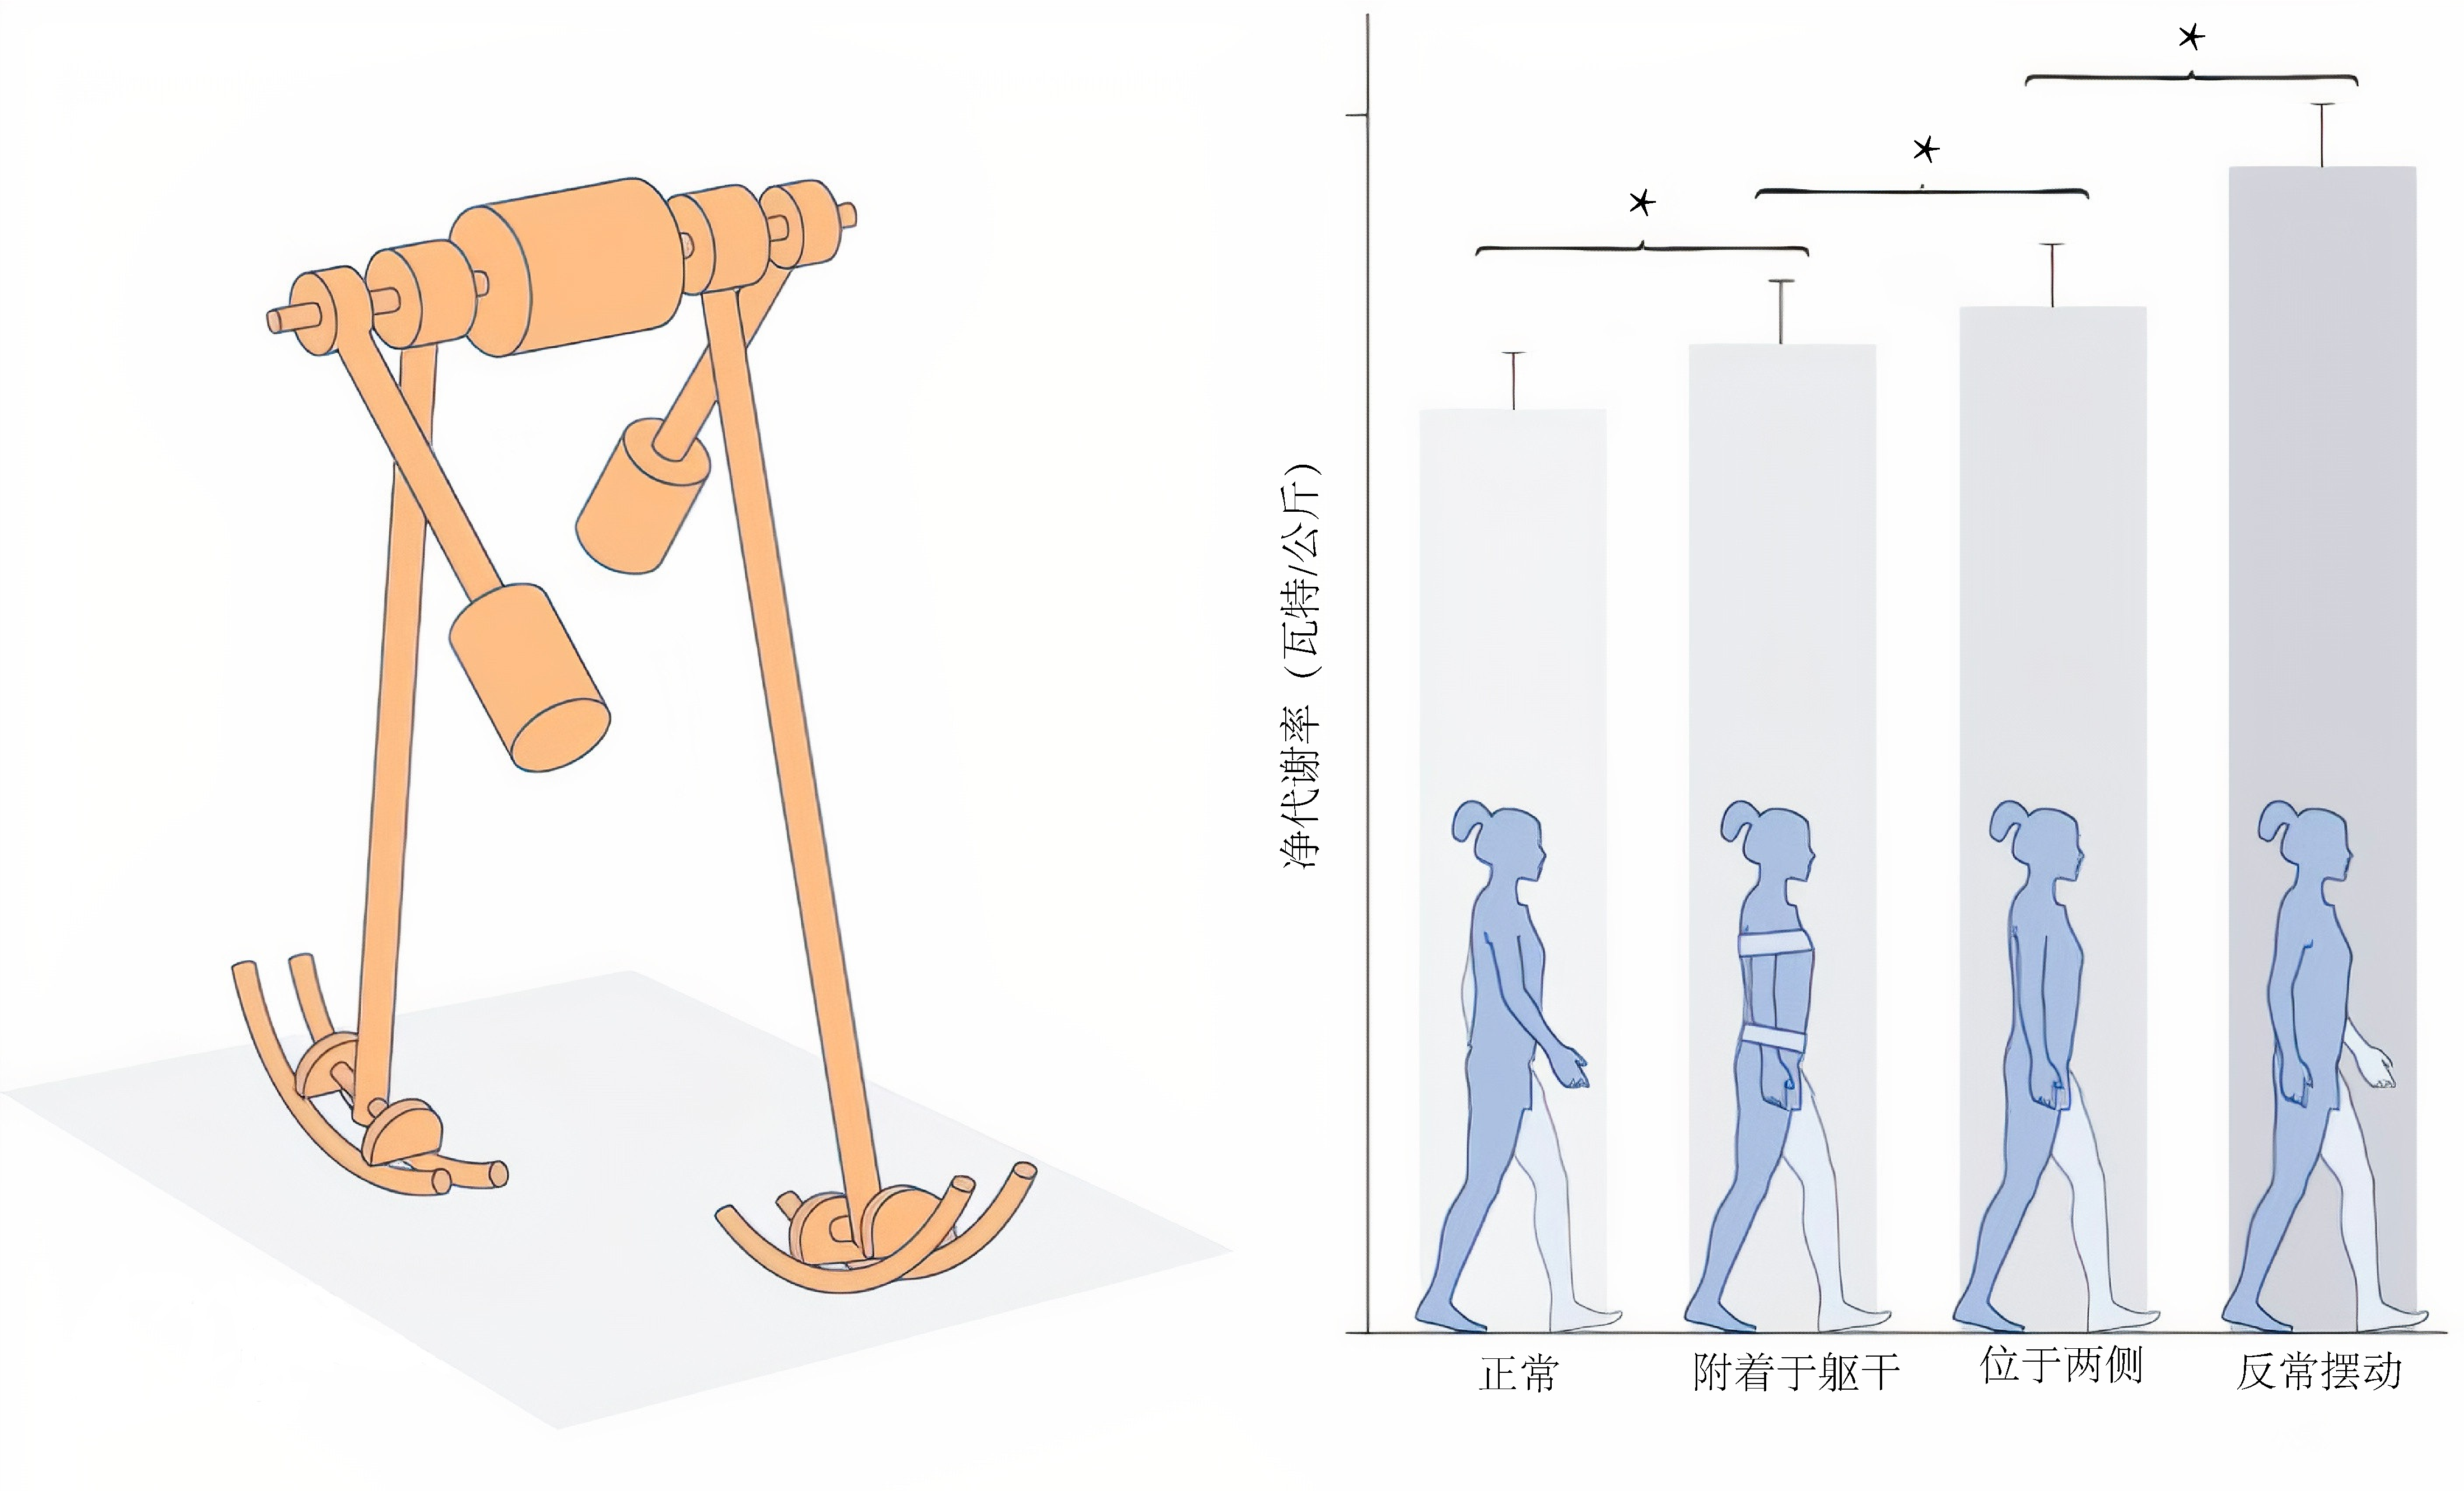
\includegraphics[width=1.0\linewidth]{chap2/2_16}
	\caption{正常和反常手臂摆动在被动行走机制中自发出现(左图)。
		在人体实验中,正常手臂摆动时能量消耗最少,反常手臂摆动时能量消耗最高(右图;误差线和星号表示标准差和统计学显著差异)\cite{collins2009dynamic}。 \label{fig:2_16}}
\end{figure}


对正常行走的人类受试者进行的实验表明,肩关节和肘关节肌肉的活性较低,这证实了正常的手臂摆动主要是被动的。
下肢的运动学和动力学不受手臂摆动策略的影响,但当手臂不摆动时,整个身体会绕垂直轴旋转得更大,而在反常手臂摆动时,旋转幅度更大。
角动量的增加被绕垂直轴更高的地面反作用力矩所抵消,从而导致肌肉活性和能量消耗相应增加。
简而言之,Bro步法很不协调,这就是为什么超过一定年龄的人通常不会这样走路。


\section{用于步态分析的骨骼模型}

由于被动步行器的每个仿生特征都提升了其性能,人们自然会好奇一个更高保真度的模型会是什么样子。
让我们先来听听一些坏消息:
解剖关节非常复杂,相邻的身体部位会在各个方向上相对平移和旋转。
我们通常只关注这些运动中的一小部分,或者只能精确测量它们。
因此,即使是刻意模仿人体的模型也会做出一些简化的假设,例如不允许股骨头和骨盆之间的相对平移,从而将髋关节表示为球窝关节。


尽管如此,图~\ref{fig:2_17}~展示了一个用于分析步态的典型且相当准确的下肢骨骼模型。(必要时可添加躯干和手臂。)
该模型由 9 个关节刚体组成:骨盆、左右股骨、髌骨、胫腓骨(小腿)和足部。
该模型的下肢有 16 个自由度:6 个自由度描述骨盆相对于固定参考系的位置和方向(倾斜、侧倾和旋转),5 个自由度描述每条腿的姿势(髋屈曲、内收和旋转;膝关节伸展;踝关节背屈)。
这些术语是标准术语,值得学习,如图~\ref{fig:2_16}~所示。

\begin{figure}[!htb]
	\centering
	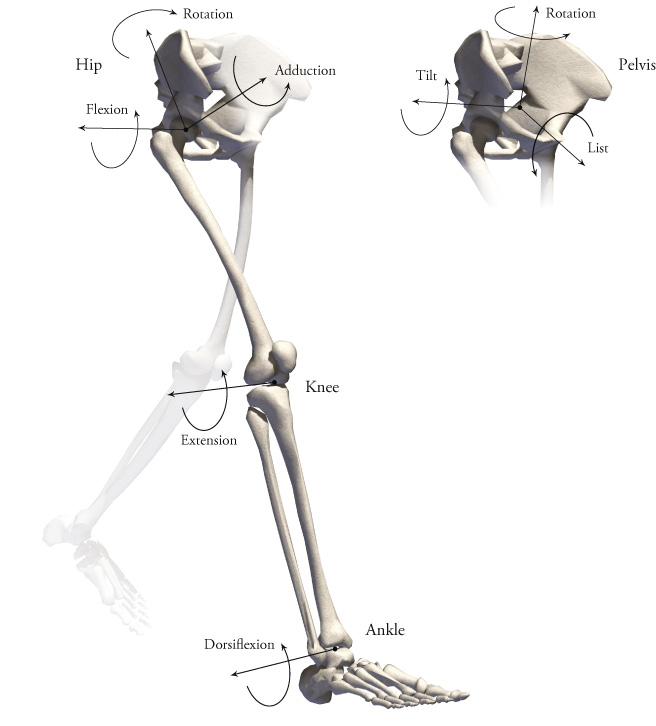
\includegraphics[width=1.0\linewidth]{chap2/2_17}
	\caption{步态分析中使用的示例模型。
		该模型包含代表骨盆、大腿、小腿和足部的刚体,仅允许在典型步态分析中可靠测量的关节运动:
		骨盆倾斜、侧倾和旋转;髋关节屈曲、内收和旋转;膝关节伸展;以及踝关节背屈\cite{rajagopal2016full}。 \label{fig:2_17}}
\end{figure}


想一想:在我们行走的每一刻,我们都在不知不觉中同时控制着十几个角度位置。
相比之下,莫洪和麦克马洪的弹道行走模型只有3个自由度,动态行走模型也只有几个自由度。
我们之所以成功,部分原因在于我们走捷径,尽可能地使用被动运动,但也因为我们的大脑在生命的第一年花费了大量时间学习如何协调复杂的行走动作。
下次你再开玩笑说有人不能一边走路一边嚼口香糖时,请记住,即使是第一步——双足行走——也是一项了不起的成就。


请注意,图~\ref{fig:2_17}~所示的模型是三维的。
正如我们所见,行走是一种三维活动,必须分析非矢状面的运动和力才能理解平衡和体重支撑。
有多种方法可以测量这些三维运动,我们将在第 7 章中介绍。
我们可以使用这些方法来估计人类受试者在行走过程中的运动,我们将在下文中介绍。


\section{步行运动学}

行走时,骨盆会经历复杂的运动(图~\ref{fig:2_18})。
在额状面上,由于肢体在站立初期负重,骨盆会向摆动侧向下倾斜。
该运动的范围几乎翻倍,从低速行走时的约 5 度增加到高速行走时的约 10 度。
在横切面上,骨盆向前进肢旋转;
因此,前肢的髋部位于后肢的髋部前方。
该运动也会随着速度的增加而增强,并提供了一种增加步长的机制。


\begin{figure}[!htb]
	\centering
	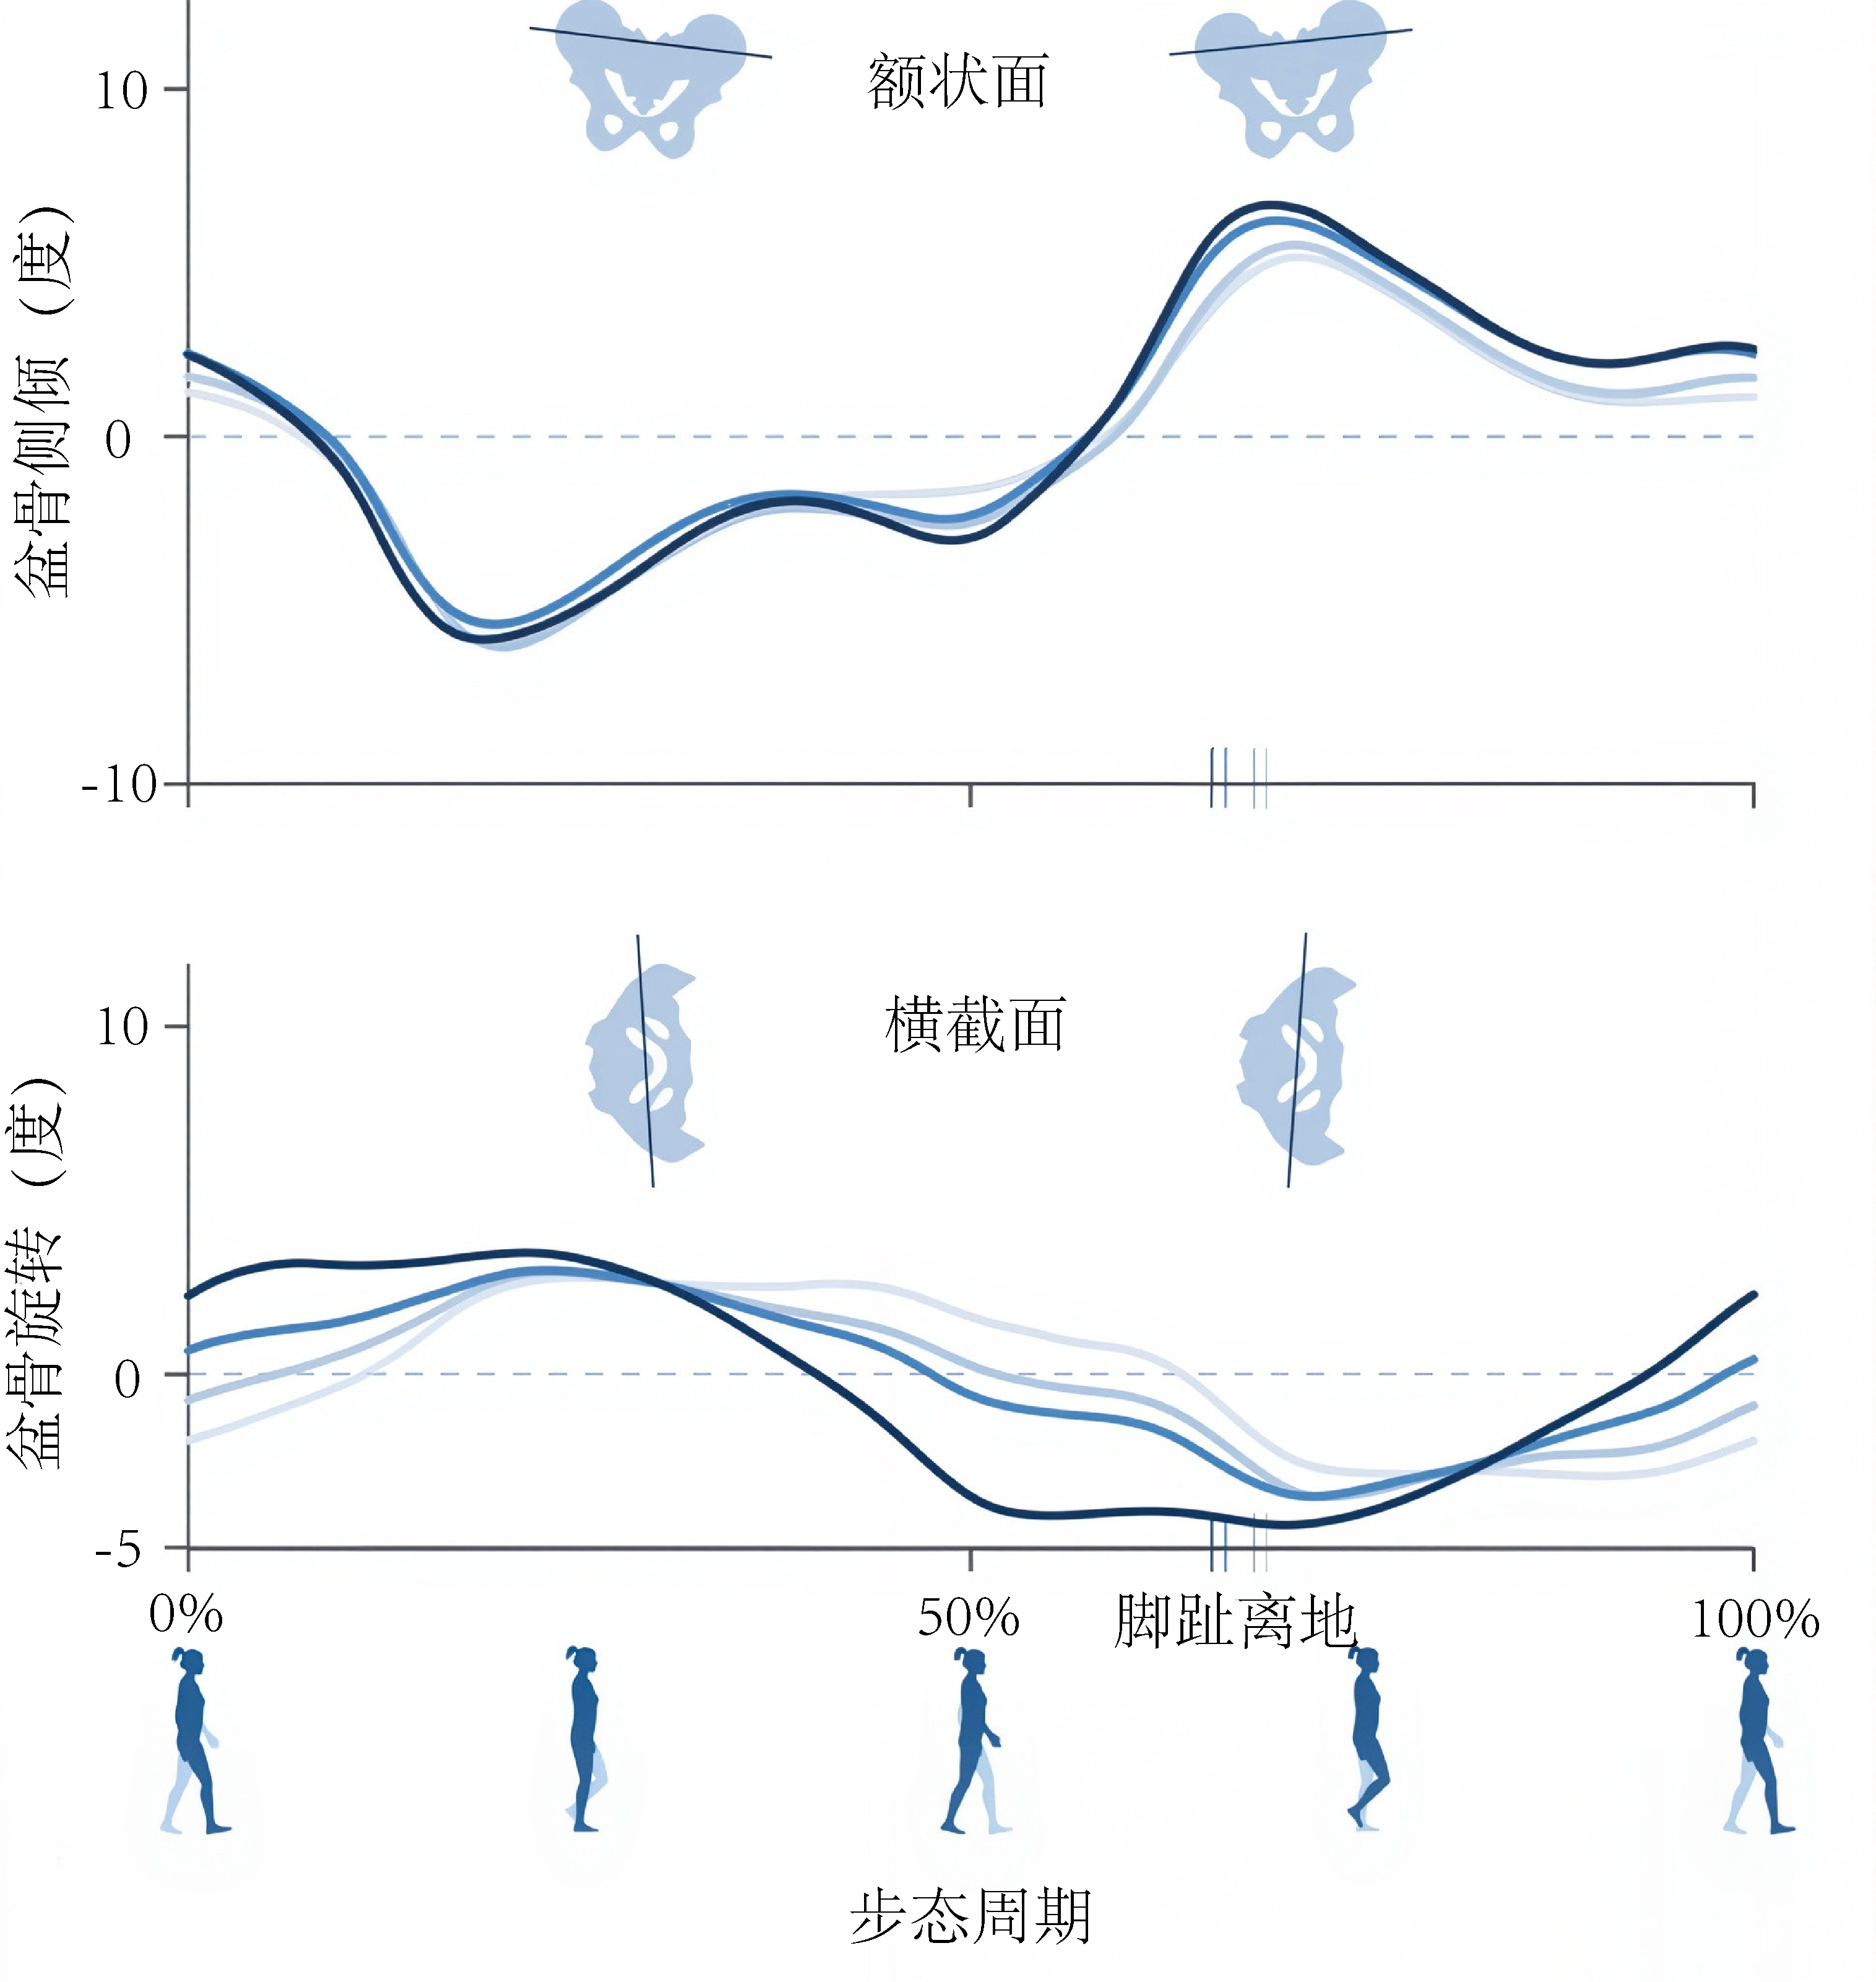
\includegraphics[width=0.8\linewidth]{chap2/2_18}
	\caption{不同速度下行走时,步态周期内骨盆的代表性方向。
		取10名受试者的平均值。
		横轴上的垂直线表示每种速度下的脚趾离地情况\cite{arnold2013muscle}。 \label{fig:2_18}}
\end{figure}


下肢关节也以典型的模式运动(图~\ref{fig:2_19})。
足触地时,髋关节处于屈曲状态。
在站立期,髋关节伸展,在足尖离地前达到最大伸展度,然后在摆动期屈曲。
足触地时,膝关节完全伸展。
当肢体负重时,膝关节像减震器一样先屈曲后伸展,速度越快,屈曲度越大。
在摆动前,膝关节快速屈曲,在摆动中期附近达到最大屈曲度,然后快速伸展,在下一次足触地前达到完全伸展。
足触地时,踝关节处于中立位。
在站立初期,随着足部向地面旋转,踝关节跖屈;
当胫骨越过足部时,踝关节背屈。
在站立期接近尾声时,踝关节快速跖屈,大约在足尖离地时达到最大伸展度。
随着步行速度的增加,峰值关节角度通常会增加,而步态周期中站立的时间会减少。


\begin{figure}[!htb]
	\centering
	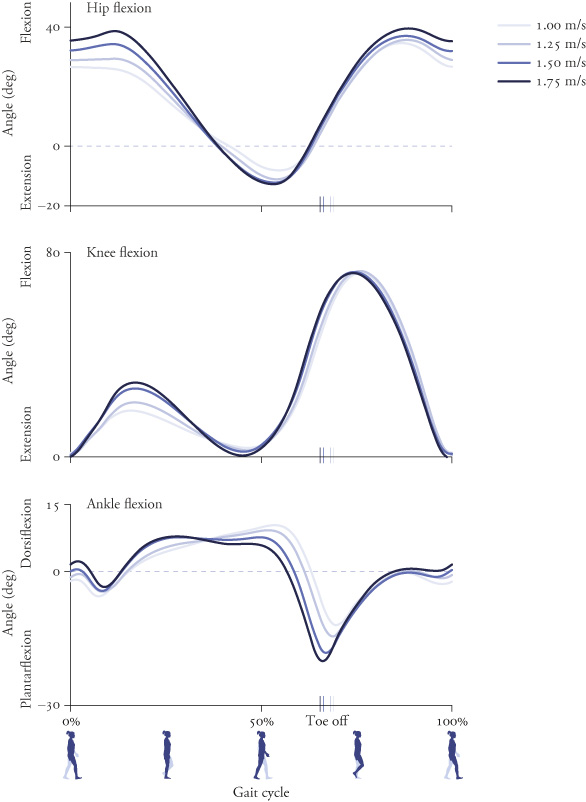
\includegraphics[width=0.9\linewidth]{chap2/2_19}
	\caption{不同速度下行走时,步态周期内的关节运动。
		取10名受试者的平均值。
		横轴上的垂直线表示每种速度下的脚趾离地情况\cite{arnold2013muscle}。 \label{fig:2_19}}
\end{figure}


\section{地面反作用力和步行速度}

图~\ref{fig:2_20}~显示了行走过程中的地面反作用力。
高速行走时,地面反作用力的垂直分量在足部触地后迅速上升,并呈现出特征性的双峰形状。
我们在图~\ref{fig:2_4}~至图~\ref{fig:2_6}~中也看到了类似的形状。
随着速度的增加,这些峰会变得更加明显。
地面反作用力的第一个峰来自支撑身体重量的前肢肌肉。
地面反作用力的第二个峰来自蹬地时后肢肌肉。
这些反作用力有助于我们了解重心的加速度,但仅凭实验无法告诉我们哪些肌肉负责产生测量到的地面反作用力。
我们将在第~\ref{chap:chap11}~章中研究肌肉如何协调行走并产生地面反作用力。


\begin{figure}[!htb]
	\centering
	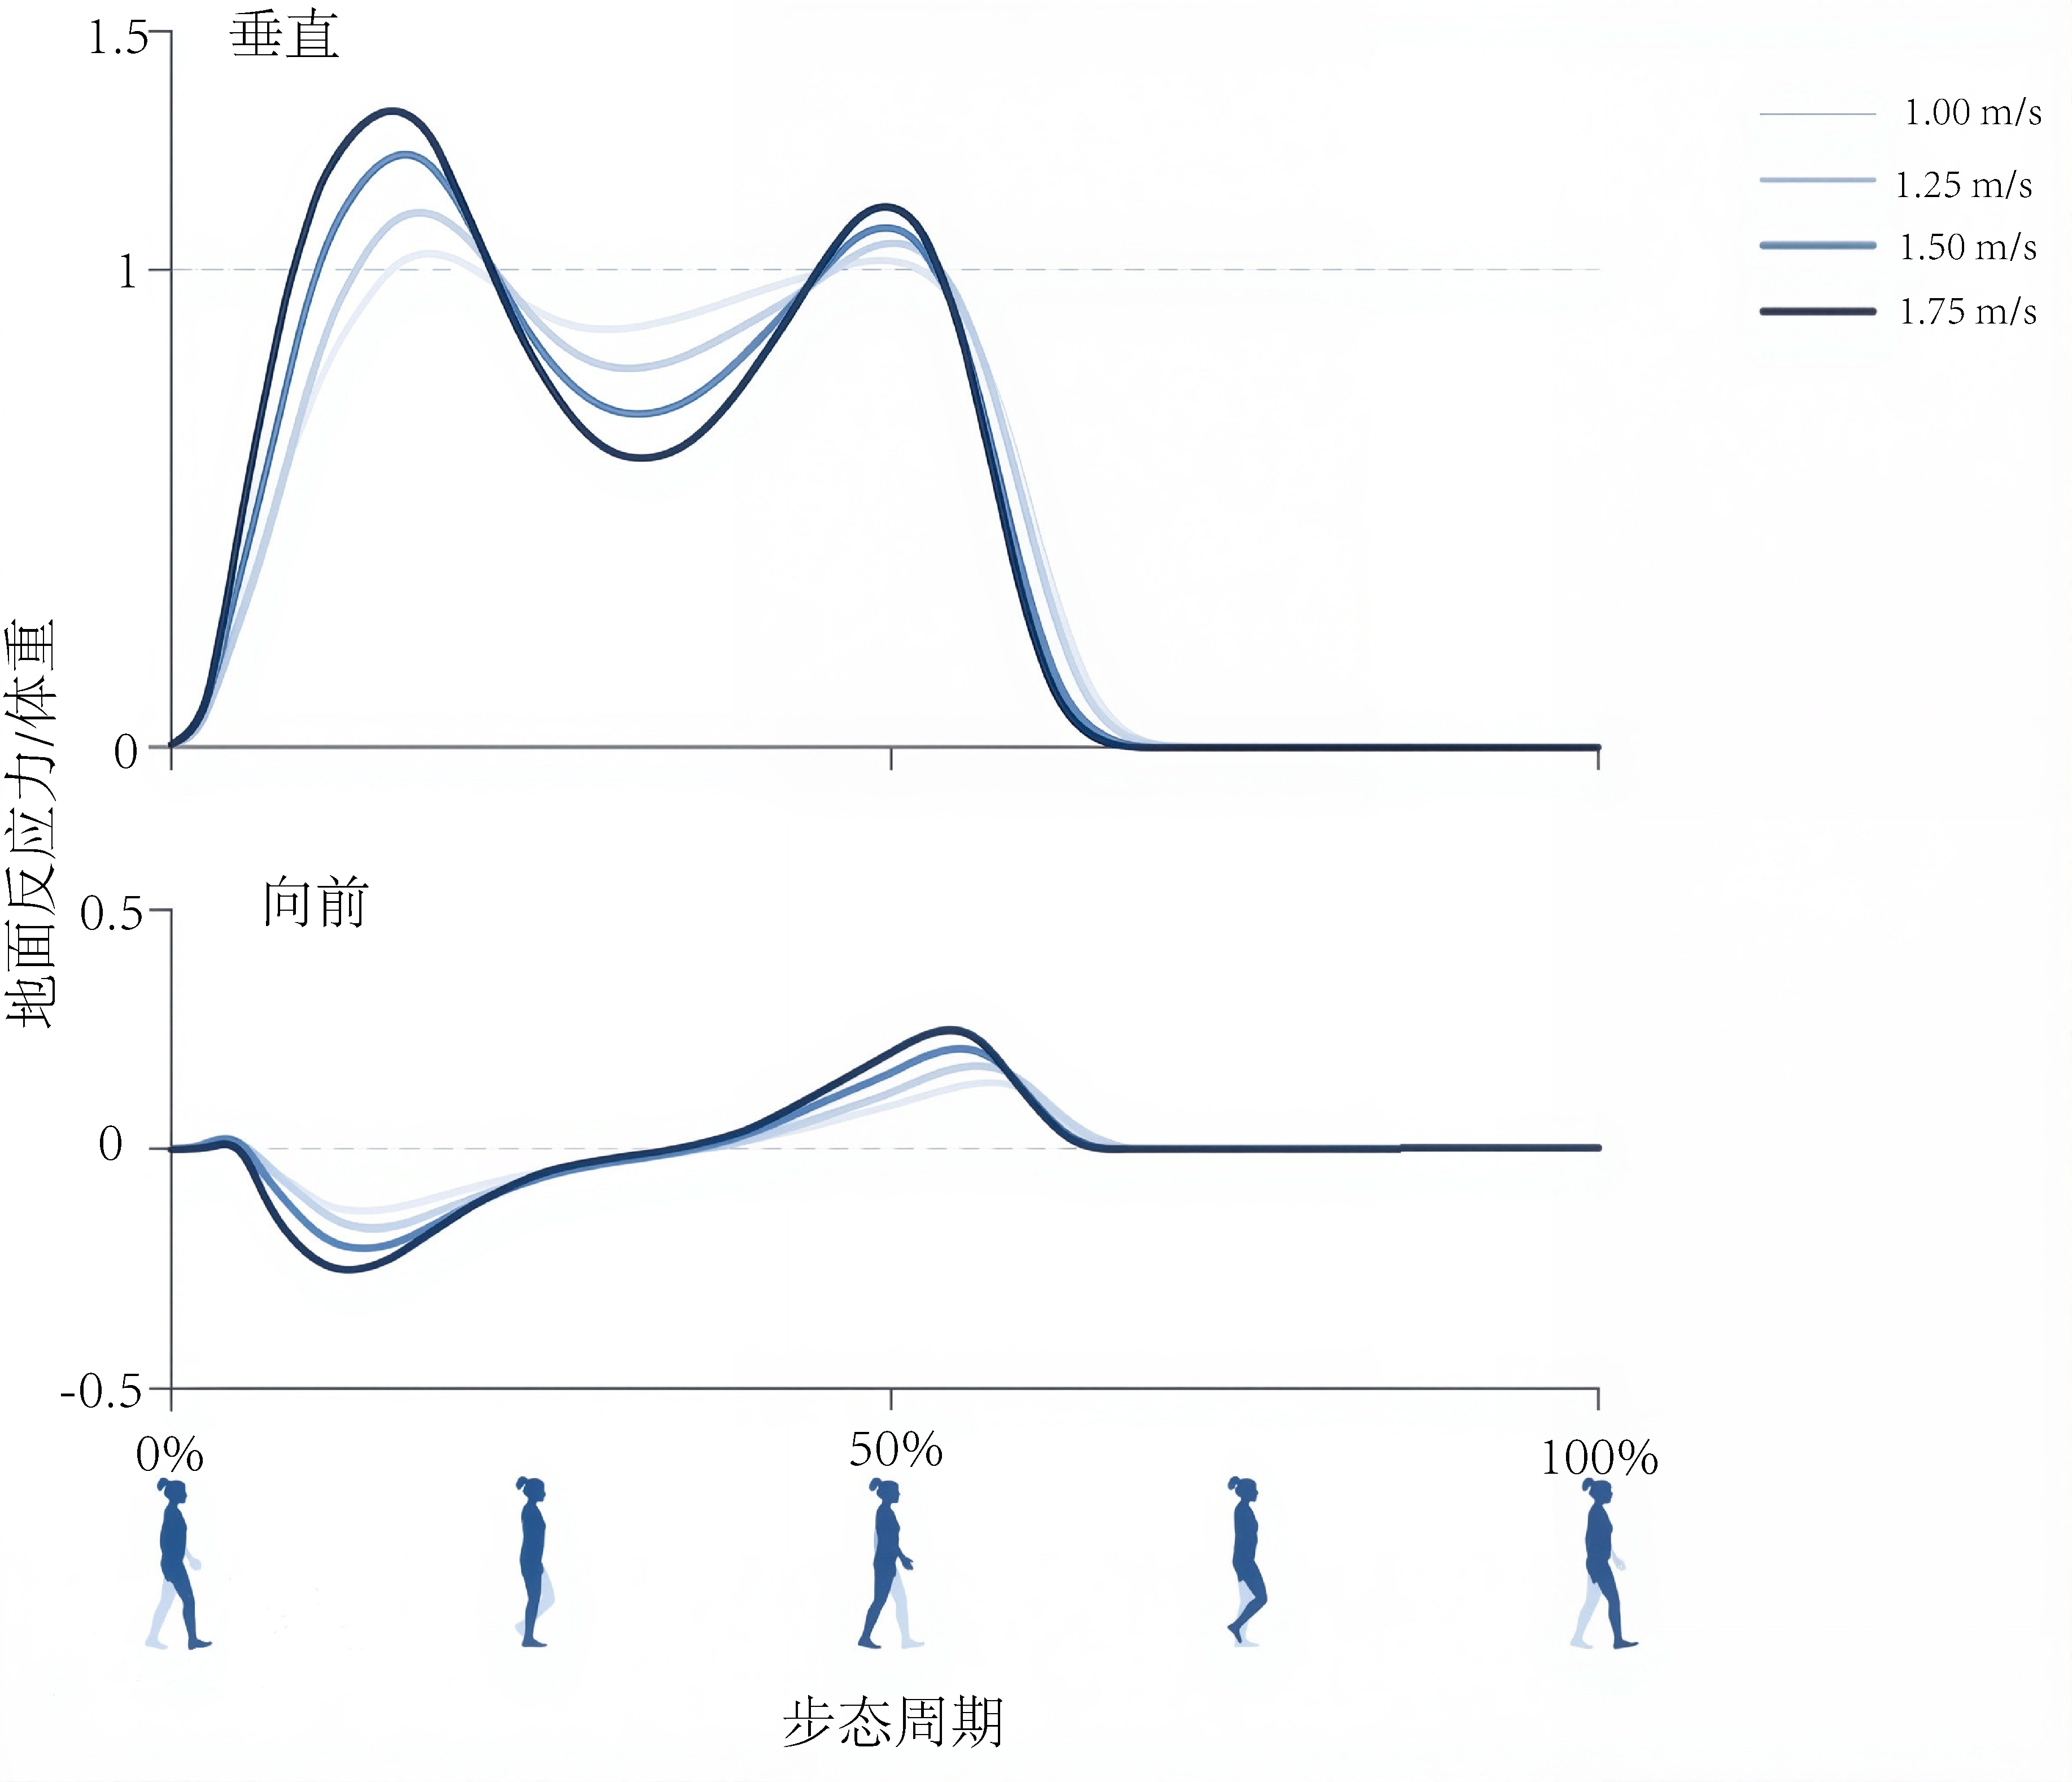
\includegraphics[width=0.95\linewidth]{chap2/2_20}
	\caption{以不同速度行走时,步态周期内代表性地面反作用力。
		已按体重标准化,并取 10 名受试者的平均值\cite{arnold2013muscle}。 \label{fig:2_20}}
\end{figure}


图~\ref{fig:2_18}–\ref{fig:2_20}所示的数据可从 \href{simtk.org}{simtk.org} 免费下载。
此类规范数据对于量化受试者的步态偏差以及测试运动模型和模拟的准确性非常有价值。


\section{非典型步态}

人类可以利用本章讨论的机制平稳高效地行走。
然而,身体或大脑的损伤以及关节或肌肉的疾病可能会扰乱行走动力学。
例如,脑瘫患者(一种因脑损伤引起的运动障碍)经常以蹲伏步态行走(图~\ref{fig:2_21})。
蹲伏步态的特点是站立期膝关节过度屈曲。
膝关节过度屈曲会带来问题,因为它会增加站立期膝关节的力量,阻碍摆动时脚趾与地面的间隙,并显著增加能量消耗(尝试以蹲伏步态行走两分钟,看看是否会气喘吁吁)。
脑瘫患者的膝关节过度屈曲通常会随着时间的推移而恶化,常常导致膝关节力学改变和慢性膝关节疼痛。
在严重的情况下,膝关节屈曲程度可能会变得非常严重,以至于患者完全丧失行走能力。


\begin{figure}[!htb]
	\centering
	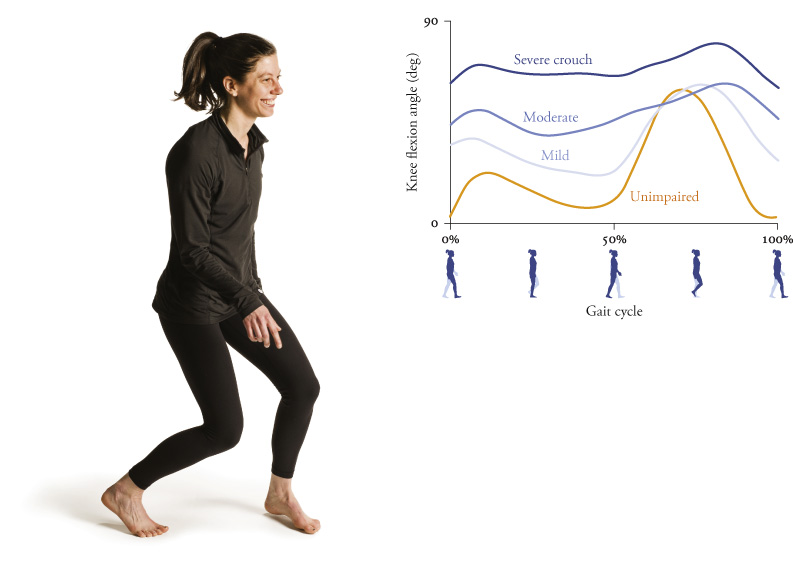
\includegraphics[width=1.0\linewidth]{chap2/2_21}
	\caption{蹲伏步态的特征是站立时膝关节过度屈曲。
		图中绘制了正常步态受试者以及脑瘫患者(轻度、中度和重度蹲伏步态)在一个步态周期内的平均膝关节屈曲角度。
		左图为Rachel Jackson演示的中度蹲伏步态行走\cite{steele2012compressive}。 \label{fig:2_21}}
\end{figure}


许多脑瘫患者以及中风患者行走时,都会出现膝关节僵硬的步态,即摆动期膝关节屈曲功能减弱且延迟(图~\ref{fig:2_22})。
这种步态还会降低脚趾与地面的距离,导致绊倒或需要进行能量效率低下的代偿性运动。
膝关节僵硬的步态被认为主要是由股直肌活动不当引起的,股直肌经髌骨穿过膝关节前方,产生膝关节伸展力矩。
因此,膝关节僵硬的步态通常采用股直肌转移术治疗,将股直肌的附着点从髌骨转移到一个能够降低其产生膝关节伸展力矩能力的部位。
遗憾的是,股直肌转移术的结果并不一致:
有些人在手术后摆动期膝关节屈曲功能有显著改善,而另一些人则几乎没有变化。


\begin{figure}[!htb]
	\centering
	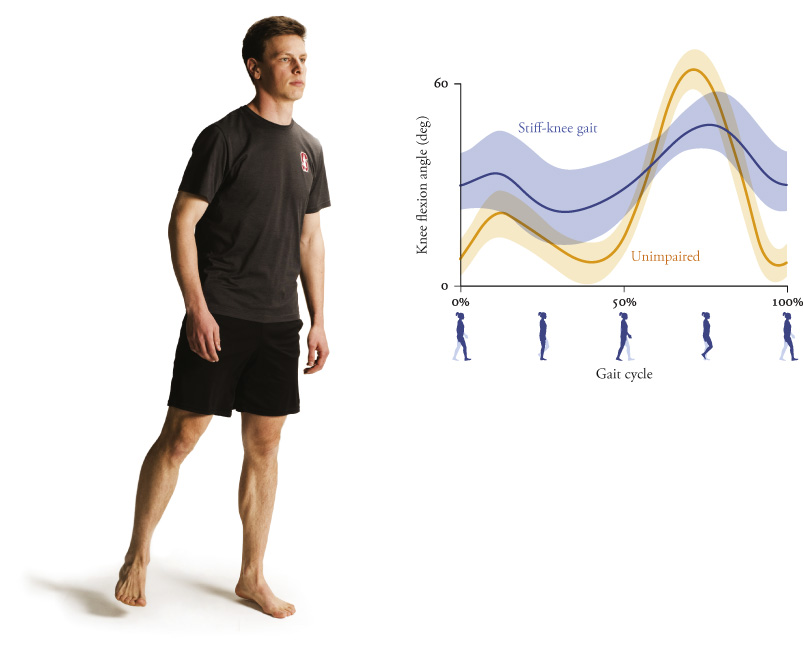
\includegraphics[width=1.0\linewidth]{chap2/2_22}
	\caption{膝关节僵硬步态的特征是摆动时膝关节屈曲减弱且延迟。
		图中显示了膝关节僵硬步态患者与未受损步态患者在步态周期内的膝关节屈曲角度(平均值±1个标准差)的比较。
		左图为Scott Uhlrich演示的膝关节僵硬步态行走\cite{fox2009mechanisms}。 \label{fig:2_22}}
\end{figure}


仅仅通过检查关节运动学,无法理解蹲伏步态或膝僵硬步态的成因,因为运动测量并不能确定导致该运动的原因。
正如我们将在第~\ref{chap:chap11}~章中看到的,肌肉驱动的步行模拟可以为理解蹲伏步态和膝僵硬步态的成因提供参考,并可用于设计有效的治疗方法。


\section{不同条件下步行的变化}

步行是一项典型的活动,这意味着我们可以从简单的模型和平均实验数据中了解到很多相关信息。
然而,并没有单一的理想步态。我们都有过仅凭走路姿势就能认出远处朋友的经历。
此外,步行方式也有很多变化,这些变化完全是针对不同情况的“正常”适应。
人们在走得慢或快、搬运杂货、爬山、参加游行或穿着高跟鞋时,步态都会有所不同。
我们还可以观察到,当佩戴经过优化以降低步行能量消耗的机器人系统时,步行动力学的变化。
表~\ref{tab:2_1}~列出了在各种条件下步行时观察到的一些变化,除下坡步行外,所有这些变化都会增加运输成本。
当然,在稳态条件下以及步态启动、转弯和加速等瞬态条件下,步行过程中还观察到了更多变化。


\begin{table}[htbp]
	\caption{在不同条件下行走时观察到的变化} \label{tab:2_1} \centering
	\begin{tabular}{cc} % l水平左居中,c水平居中
		\toprule
		条件 & 观察到的变化  \\
		\midrule
		慢 & 站立和摆动时膝关节屈曲减少,地面反作用力调节和肌肉活动减少  \\
		\midrule
		快 & 站立和摆动时膝关节屈曲增加,调节地面反作用力和肌肉活动  \\
		\midrule
		蹲伏步态 & 站立时膝关节屈曲增加,通常伴有髋关节屈曲增加  \\
		\midrule
		膝关节僵硬步态 & 摆动时膝关节屈曲峰值减少和延迟  \\
		\midrule
		足下垂 & 摆动时踝关节背屈减少  \\
		\midrule
		马蹄步态 & 站立时踝关节跖屈增加(用脚尖行走)  \\
		\midrule
		高跟鞋 & 踝关节跖屈、膝关节屈曲及支撑肢负荷率增加  \\
		\midrule
		上坡 & 站立时髋部屈曲、膝部屈曲和踝部背屈增加  \\
		\midrule
		下坡 & 站立初期踝关节跖屈增加;站立后期髋关节和膝关节屈曲增加  \\
		\midrule
		路面湿滑 & 足部初次接触时的角速度、支撑肢的负荷率和步幅减小  \\
		\midrule
		背着背包 & 增加站立持续时间、站立期间的峰值屈曲角度、地面反作用力和肌肉活动  \\
		\midrule
		增加腿部重量 & 运输成本增加,肿块位置越远,运输成本增加得越多;启动摆动的肌肉活动增加  \\
		\midrule
		肥胖 & 站立时步宽、地面反作用力和矢状面净肌肉力矩增加  \\
		\midrule
		膝下假肢 & 站立初期和中期髋部伸肌活动增加  \\
		\bottomrule
	\end{tabular}
\end{table}


人类是高效的步行者。
在最好的情况下,我们只需向前跌倒,然后迈步来避免跌倒,并注入少量能量来过渡步伐并摆动双腿。
然而,许多情况下,步行功能受损,这可能会限制日常生活活动。
步行是数十亿人的主要身体活动形式,而身体活动受限会带来严重的健康后果。
为了帮助神经系统和肌肉骨骼疾病患者恢复和改善步行能力,深入了解步行动力学至关重要。
本章只是触及皮毛。
稍后,我们将探讨正常和受损步行状态下肌肉的活动。
现在,我们先从步行过渡到跑步。













